\chapter{Results}
\label{chapt:results}
This Chapter introduces the metrics needed to evaluate and benchmark model performance, as detailed in Section \ref{sec:metrics}. Subsequently, Section \ref{sec:eval} presents a thorough evaluation of the experiments conducted in \ref{sec:experiments}, including model performance and comparative~analysis.


\section{Metrics}
\label{sec:metrics}
This section outlines the metrics used for evaluating trajectory prediction models. These include \gls{mse} and \gls{mae} for fundamental accuracy, \gls{fde} and \gls{ade} for positional accuracy, \gls{nlade} for non-linear trajectory segments, and \gls{fae} and \gls{aae} for directional accuracy. Details for each metric are provided in Sections \ref{eq:mse} to \ref{eq:aae}.

\subsection{Mean Squared Error}
\label{eq:mse}
\gls{mse} quantifies the average squared difference between predicted and true values. It is defined as:
\begin{align}
\setequationentry{Mean Squared Error}
    \text{MSE} &= \frac{1}{n \cdot m} \sum_{i=1}^n \sum_{j=1}^m \left( \hat{y}_{i,j} - y_{i,j} \right)^2
\end{align}

where \(\hat{y}_{i,j}\) and \(y_{i,j}\) are the predicted and actual values, respectively, for the \(i\)-th sample and \(j\)-th feature, \(n\) is the number of samples, and \(m\) is the number of features. This meassurement is also used to train the models.

\subsection{Mean Absolute Error}
\label{eq:mae}
\gls{mae} measures the average magnitude of the errors in a set of predictions, without considering their direction:
\begin{align}
\setequationentry{Mean Absolute Error}
    \text{MAE} &= \frac{1}{n \cdot m} \sum_{i=1}^n \sum_{j=1}^m \left| \hat{y}_{i,j} - y_{i,j} \right|
\end{align}

\subsection{Final Displacement Error}
\label{eq:FDE}
\gls{fde} calculates the Euclidean distance between the predicted final position and the true final position at time \(T_{\text{pred}}\):
\begin{align}
\setequationentry{Final Displacement Error}
    \text{FDE} &= \frac{1}{n}\sum_{i=1}^n \left( (\hat{y}_{T_{pred},i} - y_{T_{pred},i})^2 \right)
\end{align}
This metric is discussed in detail by Xu et al. \cite{xu2018collision}.

\subsection{Average Displacement Error}
\label{eq:ADE}
\gls{ade} measures the mean squared error over all predicted points in the trajectory:
\begin{align}
\setequationentry{Average Displacement Error}
    \text{ADE} &= \frac{\sum_{i=1}^n \sum_{t=T_{\text{obs}}+1}^{T_{\text{pred}}} \left( (\hat{y}_{t,i} - y_{t,i})^2 \right)}{n \cdot (T_{\text{pred}} - (T_{\text{obs}} + 1))}
\end{align}
This metric is also discussed by Xu et al. \cite{xu2018collision}.

\subsection{Average Non-Linear Displacement Error}
\label{eq:nl-ade}
\gls{nlade} focuses on the MSE in non-linear regions of a trajectory, calculated as:
\begin{align}
\setequationentry{Non-Linear Average Displacement Error}
    \text{NL-ADE} &= \frac{\sum_{i=1}^n \sum_{t=T_{\text{obs}}+1}^{T_{\text{pred}}} I_{t,i}  (\hat{y}_{t,i} - y_{t,i})^2}{\sum_{i=1}^n \sum_{t=T_{\text{obs}}+1}^{T_{\text{pred}}} I_{t,i}}
\end{align}

where \(I_{t,i}\) is an indicator function that equals 1 if the trajectory has a non-zero curvature at time \(t\) and 0 otherwise \cite{xu2018collision}. Human movements are dynamic and continuously changing. To make \gls{nlade} useful, it is necessary to introduce a threshold, for example, \(\delta v = 0.5 \text{m/s}\). Trajectories with curvature below this threshold would be considered not non-linear enough.

\subsection*{Angular Error}
\label{eq:angular error}
\gls{ae} quantifies the discrepancy between the predicted and true velocity vectors. It can be measured using the cosine similarity, defined as:
\begin{align}
\setequationentry{Cosine Similarity}
    \cos \theta_{t,i} &= \frac{\mathbf{v}_{t,i} \cdot \hat{\mathbf{v}}_{t,i}}{\|\mathbf{v}_{t,i}\| \|\hat{\mathbf{v}}_{t,i}\|} \\
\setequationentry{Angular Error}
\label{angular_error}
    \theta_{t,i} &= \text{arccos} \left( \frac{\mathbf{v}_{t,i} \cdot \hat{\mathbf{v}}_{t,i}}{\|\mathbf{v}_{t,i}\| \|\hat{\mathbf{v}}_{t,i}\|} \right)
\end{align}

where \(\mathbf{v}_{t,i}\) and \(\hat{\mathbf{v}}_{t,i}\) are the true and predicted velocity vectors, respectively, at time \(t\). For numerical stability, a small \(\epsilon\) is added to the denominator.


\subsection{Final Angular Error}
\label{eq:fae}
\gls{fae} measures the angular discrepancy at the final time step \(T_{\text{pred}}\). It is computed as:
\begin{align}
\setequationentry{Final Angular Error}
    \text{FAE} &= \frac{1}{n} \sum_{i=1}^n \left| \theta_{T_{\text{pred}},i} - \theta_{T_{\text{pred}},i}^\text{true} \right| \times \frac{180}{\pi}
\end{align}

where \(\theta_{T_{\text{pred}},i}\) is the \gls{ae} calculated at \(T_{\text{pred}}\) as defined in \eqref{angular_error}.

\subsection{Average Angular Error}
\label{eq:aae}
\gls{aae} computes the mean angular difference between predicted and true velocity vectors over all time steps. It is defined as:
\begin{align}
\setequationentry{Average Angular Error}
    \text{AAE} &= \frac{1}{n \cdot (T_{\text{pred}} - T_{\text{obs}})} \sum_{i=1}^n \sum_{t=T_{\text{obs}}+1}^{T_{\text{pred}}} \theta_{t,i} \times \frac{180}{\pi}
\end{align}

where \(\theta_{t,i}\) is the \gls{ae} calculated for trajectory \(i\) at time \(t\) as defined in \eqref{angular_error}.

These metrics offer a comprehensive assessment of trajectory prediction performance, capturing various dimensions of accuracy and error.
\FloatBarrier

\section{Experiment Evaluation}
\label{sec:eval}
This Chapter introduces the metrics needed to evaluate and benchmark model performance, as detailed in Section \ref{sec:metrics}. Subsequently, Section \ref{sec:eval} presents a thorough evaluation of the experiments conducted in \ref{sec:experiments}, including model performance and comparative~analysis.

\subsection{E1: Attention-Based versus Baseline Models}

This Section introduces the results of Experiment 1 \ref{exp:e1} which incestigates the question \textbf{Q1: How do attention-based models compare to other models in general?}.
\label{exp:init}
\begin{figure}[t]
    \centering
    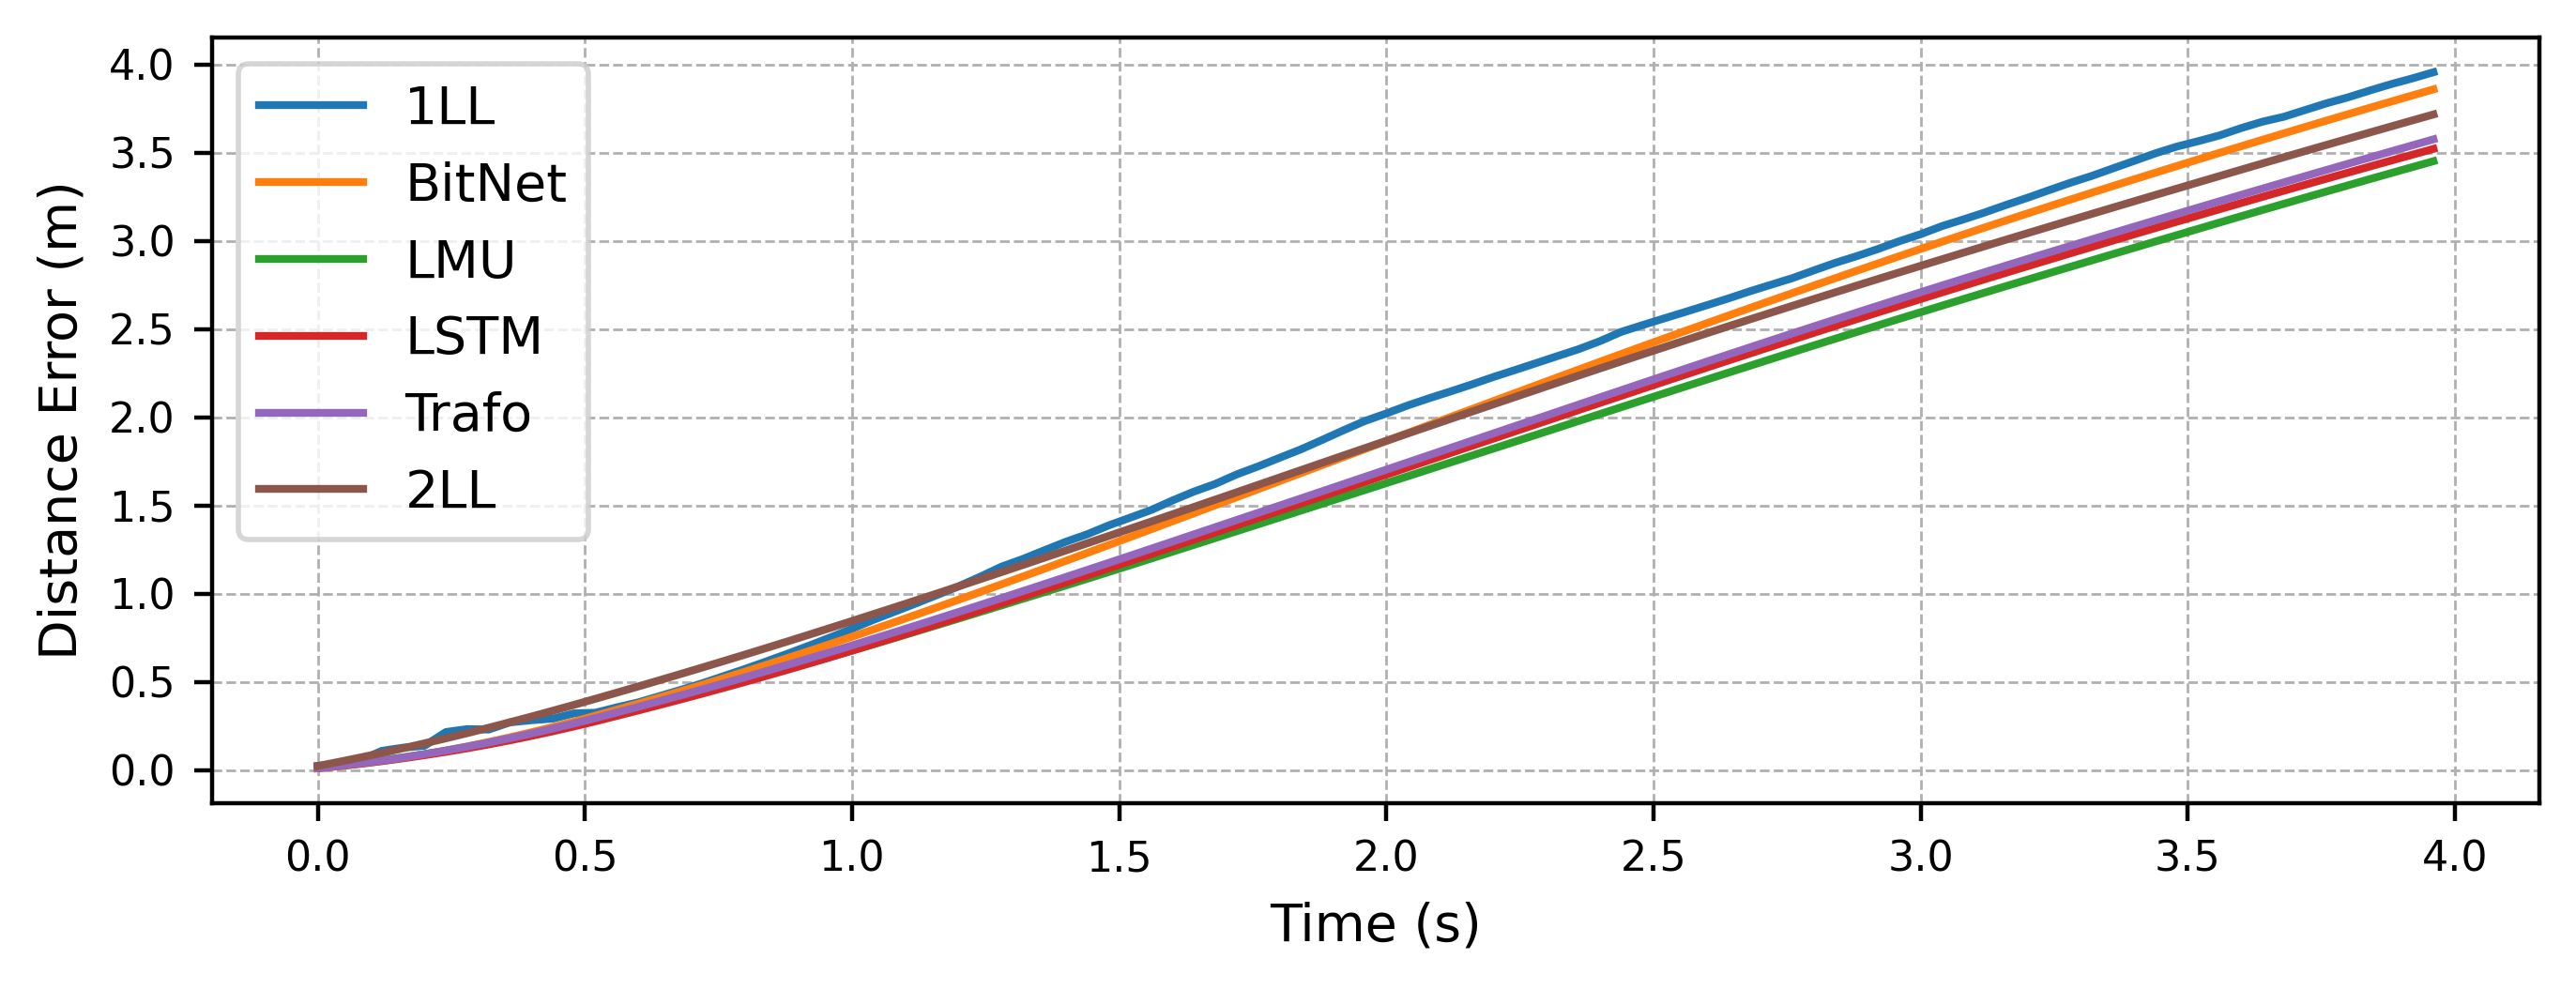
\includegraphics[width=\linewidth]{contents/results/nba_error.png}
    \caption[Distance Error Over Time (NBA).]{Plot showing the distance error over time for the NBA models, highlighting the performance trends of each model.}    \label{fig:distance_error_nba}
\end{figure}
\begin{figure}[t]
    \centering
    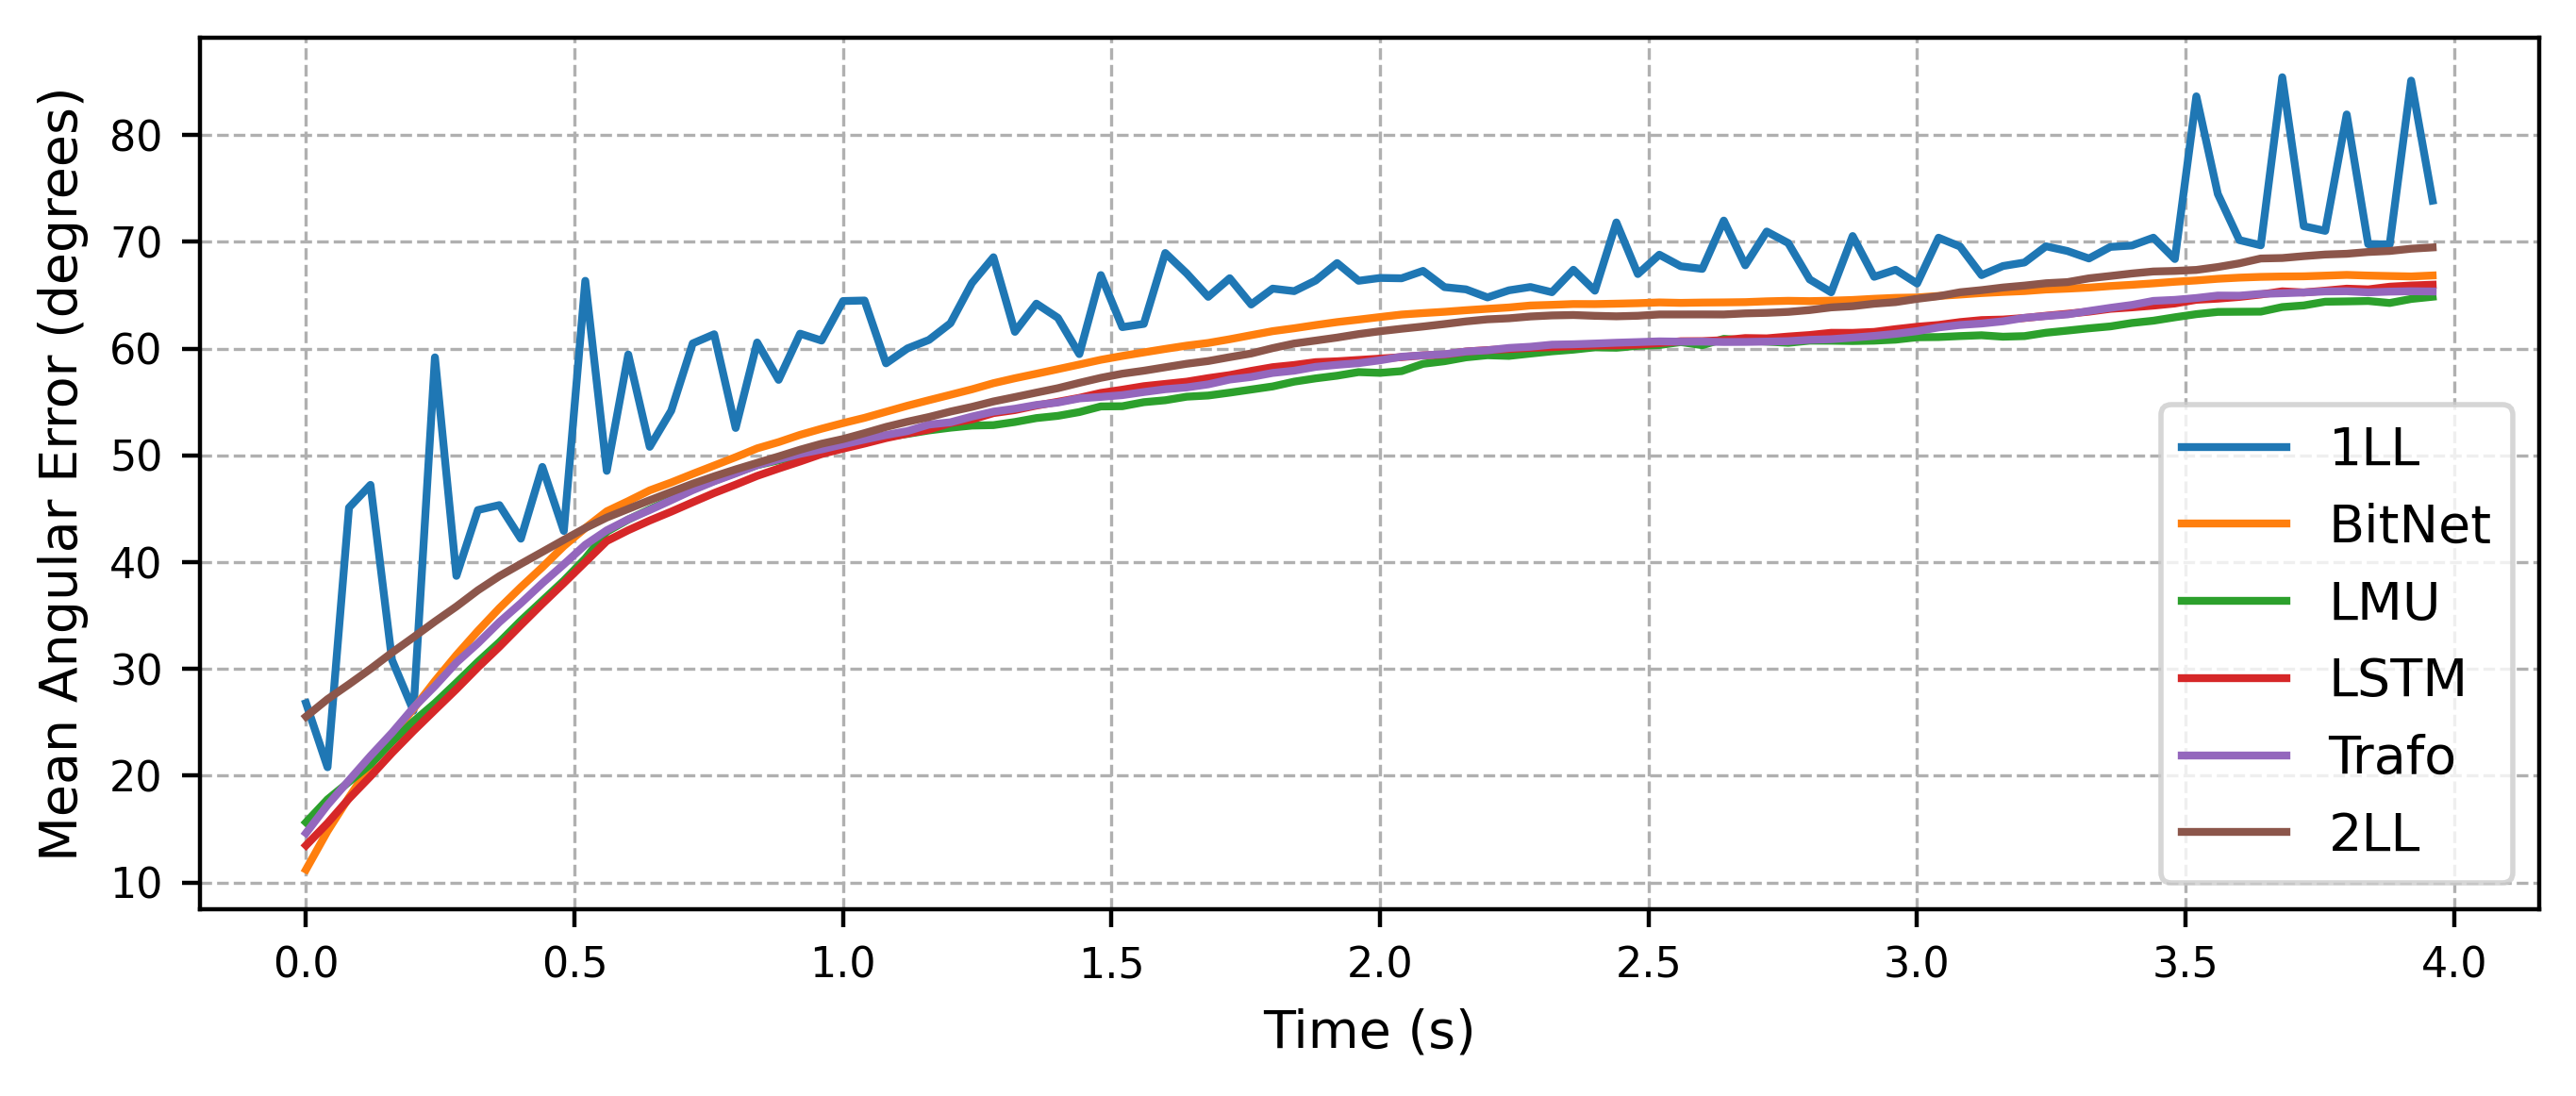
\includegraphics[width=\linewidth]{contents/results/nba_angle.png}
    \caption[Angular Error Over Time (NBA).]{Plot illustrating the angular error over time for the NBA models, demonstrating how well each model performs in this metric.}
    \label{fig:angular_error_nba}
\end{figure}
This section presents the results of Experiment E1 \ref{exp:e1} for the NBA and soccer datasets, revealing insights into the performance of attention-based models compared to established baseline models.
\paragraph{NBA Result:}

\begin{longtable}[t]{l|l||c|c|c|c|c|c}
\caption[Results of the first experiment (NBA).]{Results table for the NBA dataset, with the best scores highlighted in bold.} \label{tab:first_experiment_nba} \\

\hline
Metric & Statistic & 1L Linear & 2L Linear & BitNet & LMU & LSTM & Trafo \\
\hline\hline
\endfirsthead

\caption*{Continuation of Table \ref{tab:first_experiment_nba}} \\
\hline
Metric & Statistic & 1L Linear & 2L Linear & BitNet & LMU & LSTM & Trafo \\
\hline\hline
\endhead

\hline
\endfoot

\hline
AAE (\si{\text{grad}}) & Mean & 63.03 & 56.72 & 56.72 & \textbf{53.29} & 53.86 & 54.43 \\
 & Std & 52.14 & 50.99 & 50.99 & 49.85 & 50.42 & 50.42 \\
\hline
ADE (\si{\meter}) & Mean & 1.94 & 1.84 & 1.85 & \textbf{1.63} & 1.67 & 1.70 \\
 & Std & 1.17 & 1.23 & 1.19 & 1.11 & 1.13 & 1.16 \\
\hline
FAE (\si{\text{grad}}) & Mean & 73.91 & 69.33 & 67.04 & \textbf{64.74} & 65.89 & 65.32 \\
 & Std & 51.57 & 54.43 & 52.71 & 52.14 & 52.14 & 51.57 \\
\hline
FDE (\si{\meter}) & Mean & 3.96 & 3.72 & 3.86 & \textbf{3.45} & 3.52 & 3.58 \\
 & Std & 2.57 & 2.67 & 2.59 & 2.47 & 2.55 & 2.59 \\
\hline
MAE (\si{\meter}) & Mean & 1.23 & 1.16 & 1.17 & \textbf{1.03} & 1.06 & 1.08 \\
 & Std & 0.74 & 0.77 & 0.75 & 0.70 & 0.71 & 0.73 \\
\hline
MSE (\si{\meter}) & Mean & 3.76 & 3.57 & 3.60 & \textbf{2.92} & 3.06 & 3.18 \\
 & Std & 5.20 & 5.10 & 5.19 & 4.88 & 4.95 & 5.02 \\
\hline
NL\_ADE (\si{\meter}) & Mean & 2.34 & 2.35 & 2.36 & \textbf{2.14} & 2.18 & 2.21 \\
 & Std & 1.53 & 1.62 & 1.58 & 1.53 & 1.55 & 1.55 \\
\hline
\end{longtable}

\FloatBarrier

The results presented in Table \ref{tab:first_experiment_nba} indicate that the Transformer performed slightly worse than the RNN models across all metrics. Notably, the LMU outperformed the LSTM across all metrics in the NBA dataset, achieving an AAE of \SI{53.29}{\degree} and an ADE of \SI{1.63}{\meter}. This finding highlights the LMU's effectiveness in capturing the complexities of motion forecasting, which may stem from its ability to better model long-range dependencies compared to LSTM. In contrast, the Transformer achieved an AAE of \SI{54.43}{\degree} and an ADE of \SI{1.70}{\meter}, demonstrating that while attention-based models have potential, they still struggle with the inherent temporal dynamics of basketball, where rapid changes~occur.

Additionally, the linear models, including 1L Linear and 2L Linear, performed among the worst, with the 1L Linear model being particularly unstable as notable in the table for Mean Angular Error. The BitNet model also underperformed significantly across both datasets, which might be attributed to its limitation in encoding information using only binary values (0 and 1). This reduced capacity for nuanced information could hinder its effectiveness in the complex domain of human motion forecasting. Figures \ref{fig:distance_error_nba} and \ref{fig:angular_error_nba} illustrate the performance trends over prediction length, showing that all models exhibited a decline in accuracy as the prediction length increased, which aligns with expectations in the domain of human motion forecasting. This behavior underscores the challenges inherent in accurately predicting future positions over extended timeframes.

\newpage
\paragraph{Soccer Result:} 

\begin{figure}[t]
    \centering
    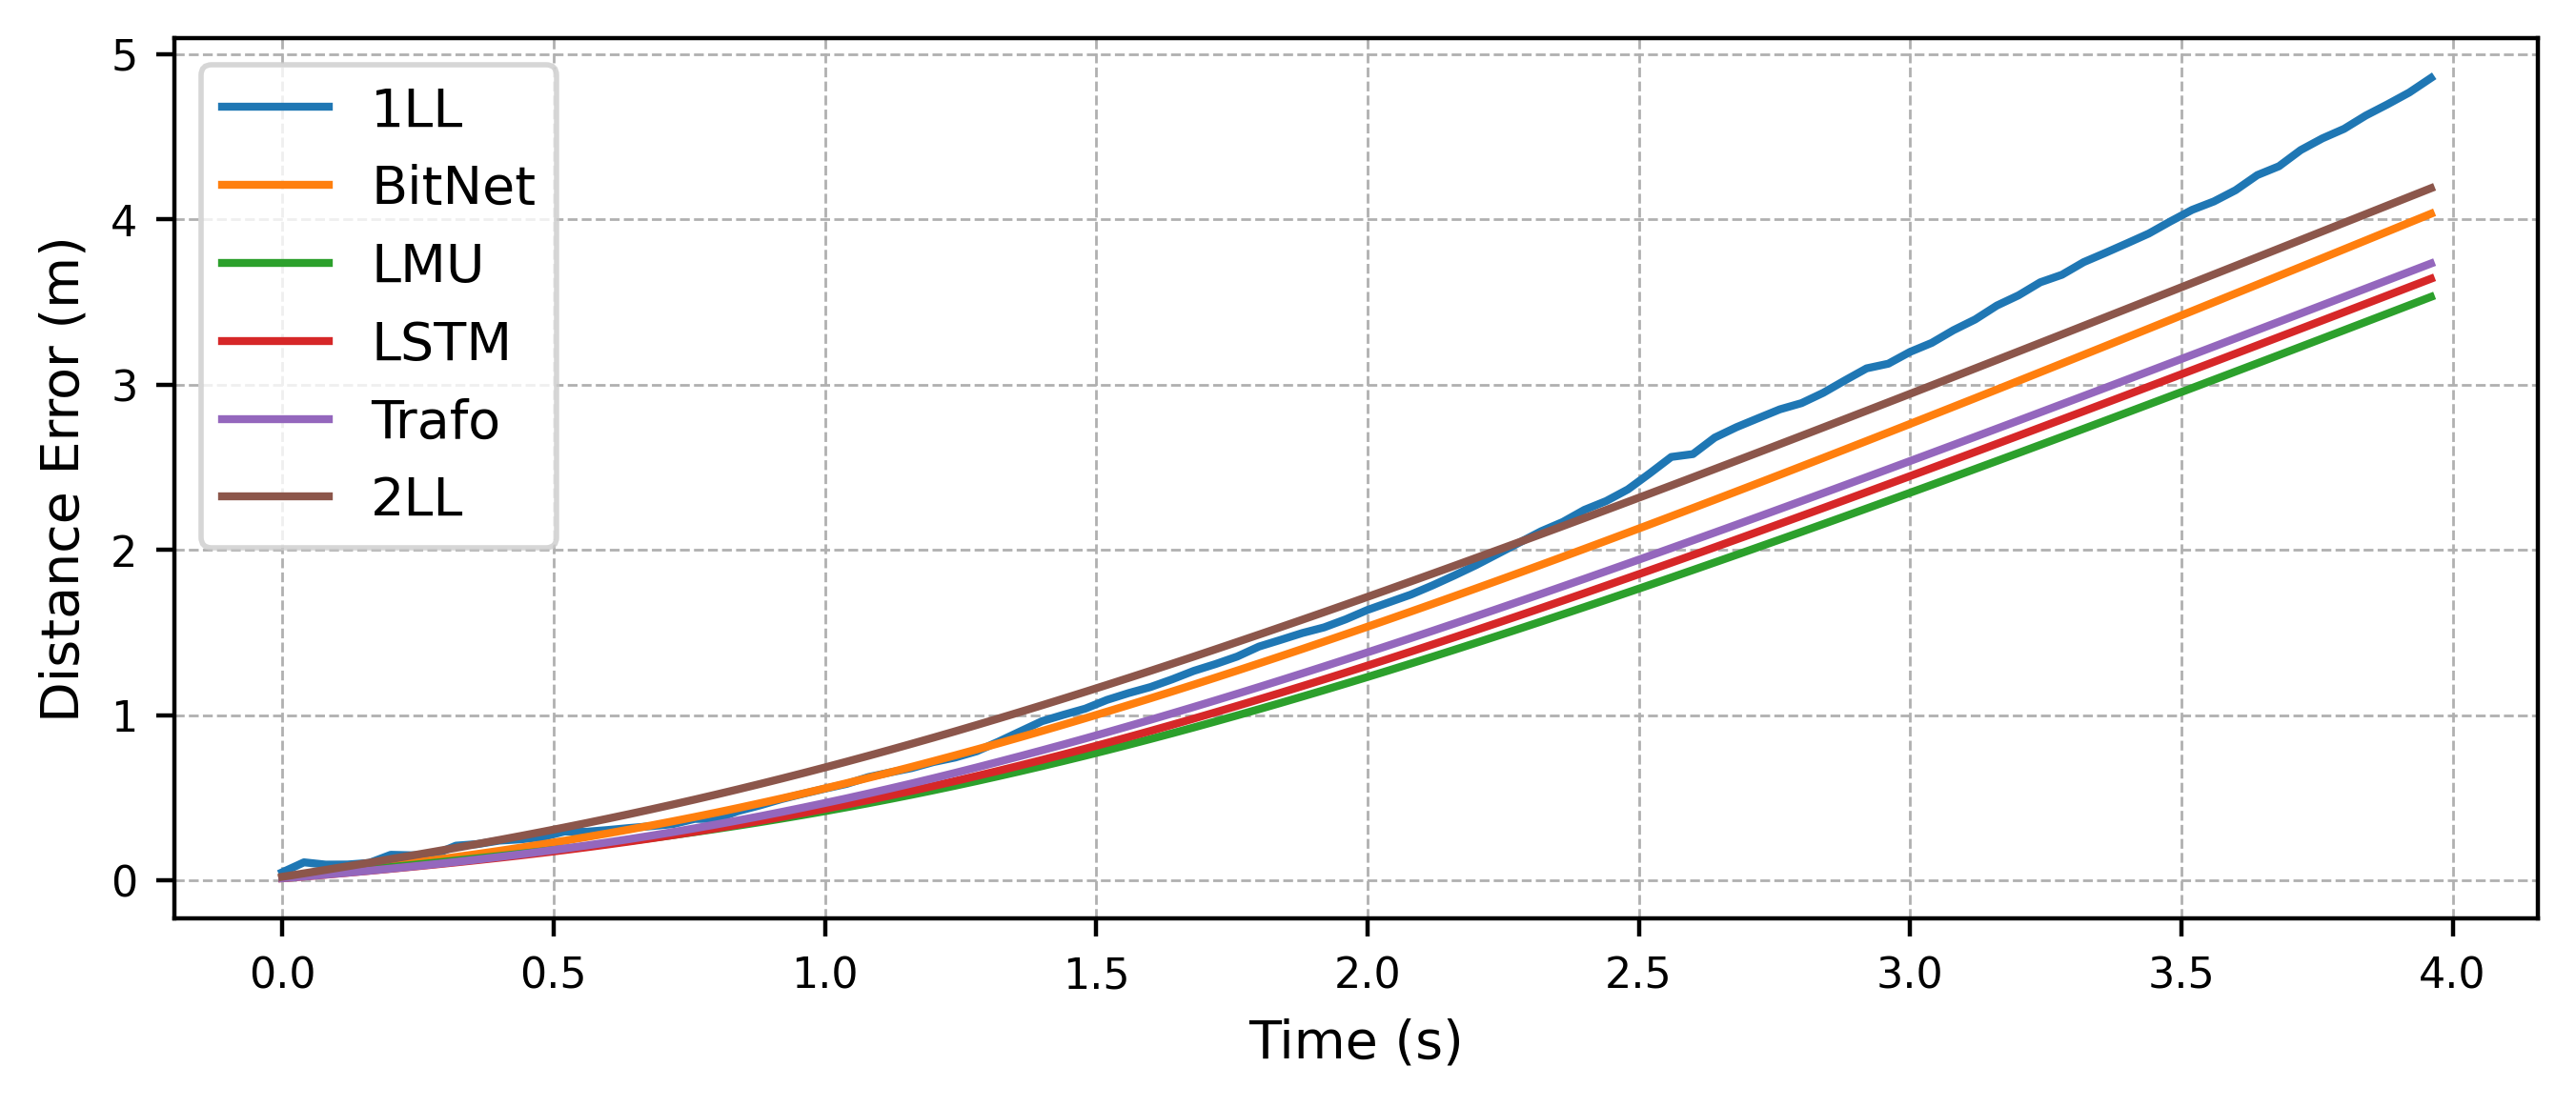
\includegraphics[width=\linewidth]{contents/results/soccer_error.png}
    \caption[Distance Error Over Time (DFL).]{Plot showing the distance error over time for the DFL models, highlighting the performance trends of each model.}
    \label{fig:distance_error_dfl}
\end{figure}
\begin{figure}[t]
    \centering
    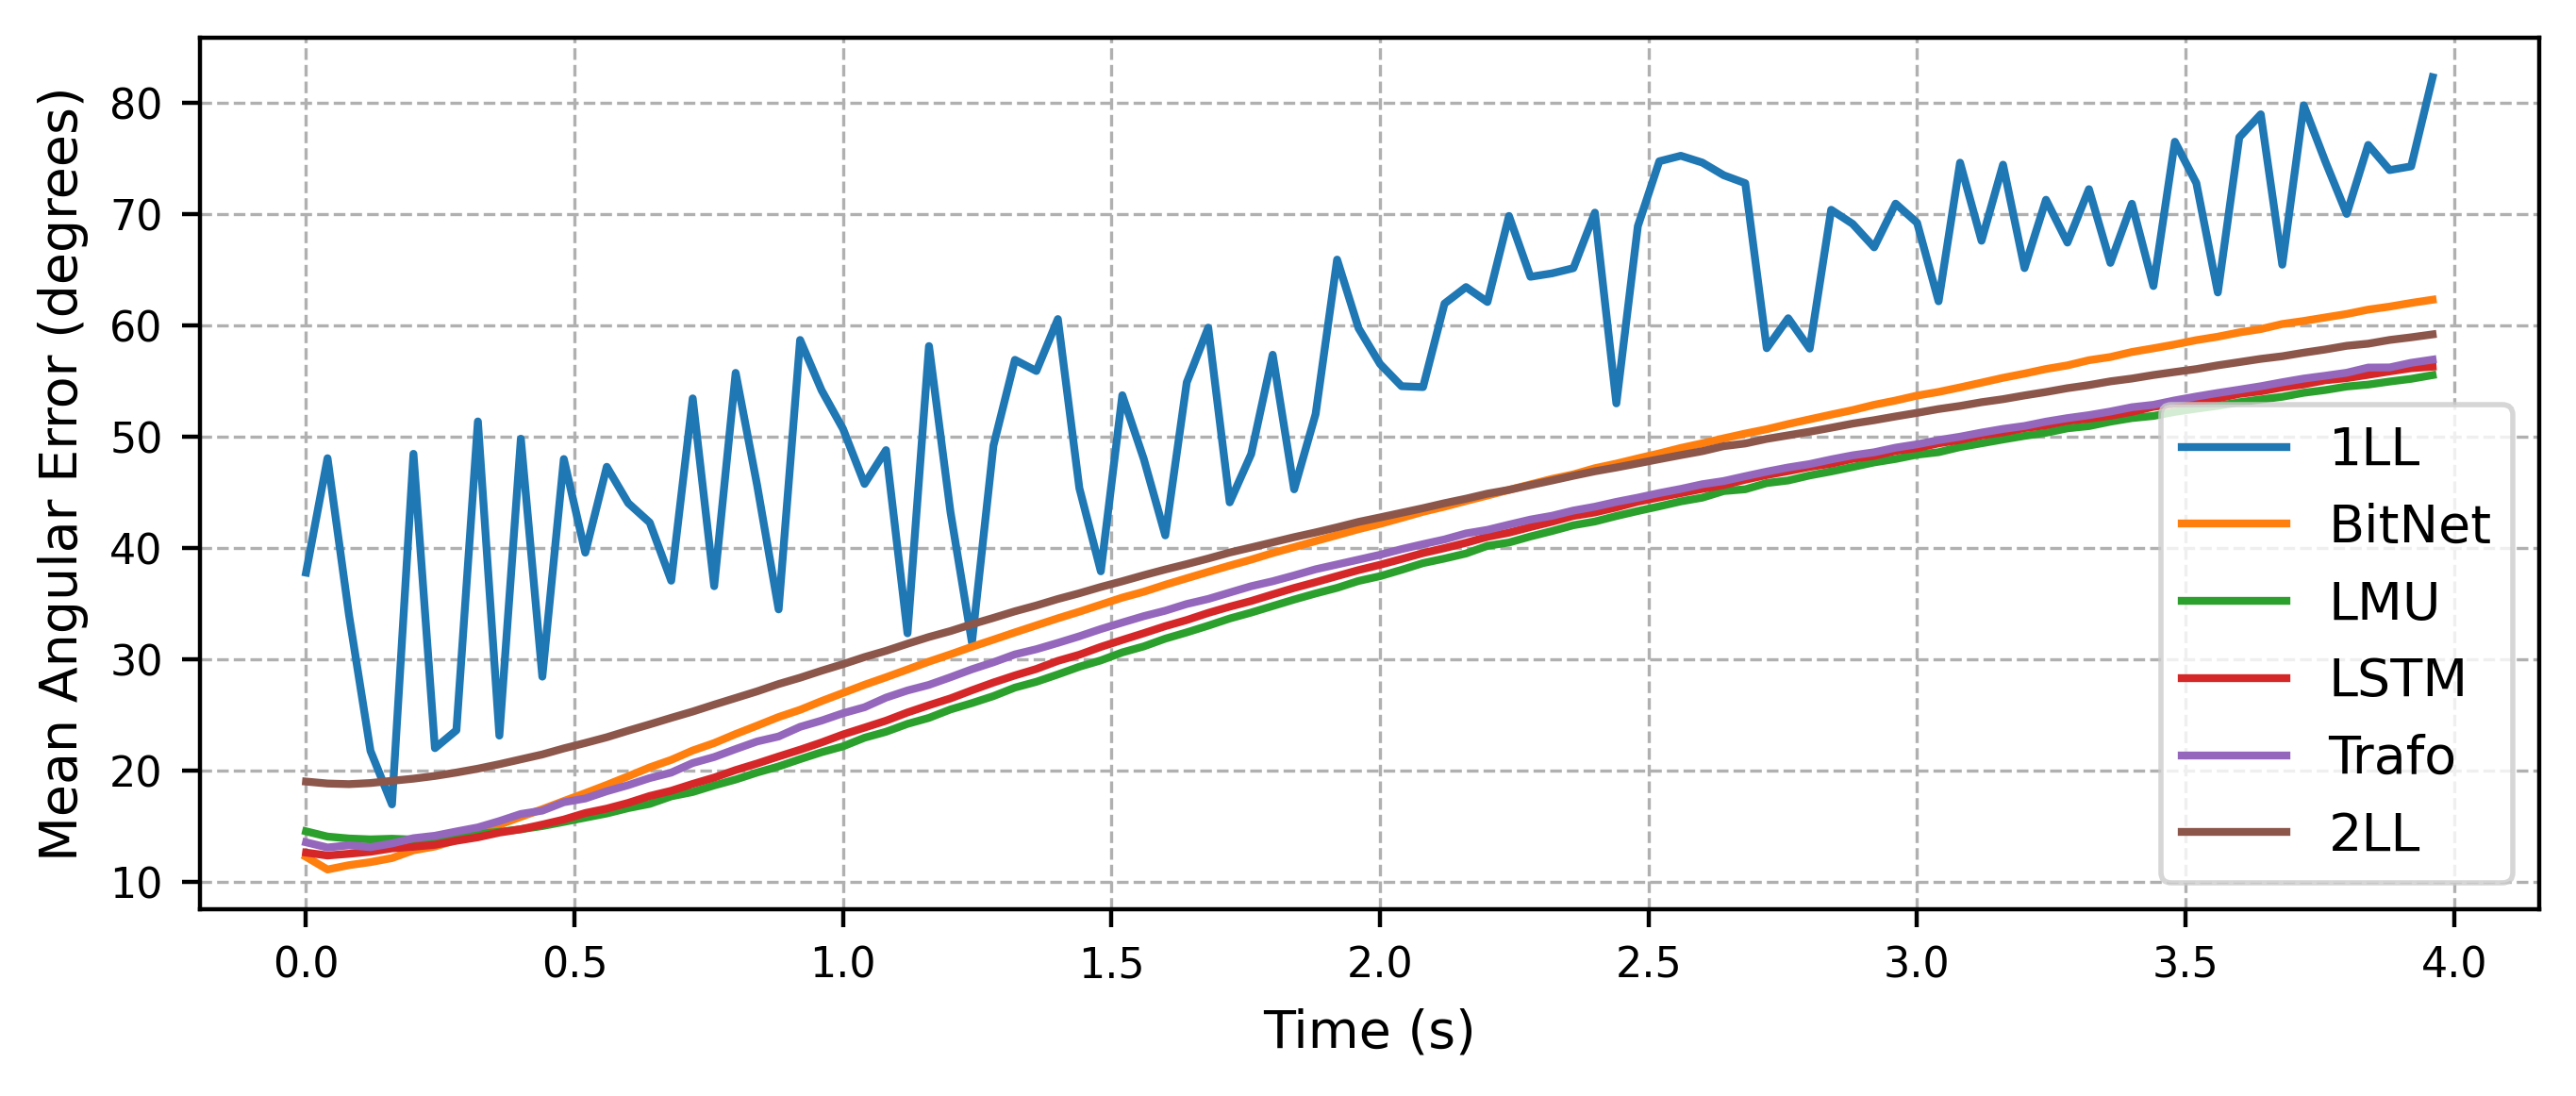
\includegraphics[width=\linewidth]{contents/results/soccer_angle.png}
    \caption[Angular Error Over Time (DFL).]{Plot illustrating the angular error over time for the DFL models, demonstrating how well each model performs in this metric.}
    \label{fig:angular_error_dfl}
\end{figure}


\begin{longtable}[t]{l|l||c|c|c|c|c|c}
\caption[Results of the first experiment (DFL).]{Results table for the DFL dataset, with the best scores highlighted in bold.} \label{tab:first_experiment_soccer} \\

\hline
Metric & Statistic & 1L Linear & 2L Linear & BitNet & LMU & LSTM & Trafo \\
\hline\hline
\endfirsthead

\caption*{Continuation of Table \ref{tab:first_experiment_soccer}} \\
\hline
Metric & Statistic & 1L Linear & 2L Linear & BitNet & LMU & LSTM & Trafo \\
\hline\hline
\endhead

\hline
\endfoot

\hline
AAE (\si{\text{grad}}) & Mean & 56.72 & 40.68 & 39.53 & \textbf{35.52} & 36.10 & 36.67 \\
 & Std & 47.56 & 42.97 & 43.54 & 41.25 & 41.83 & 41.83 \\
\hline
ADE (\si{\meter}) & Mean & 1.92 & 1.83 & 1.69 & \textbf{1.41} & 1.47 & 1.53 \\
 & Std & 1.15 & 1.29 & 1.34 & 1.02 & 1.14 & 1.17 \\
\hline
FAE (\si{\text{grad}}) & Mean & 82.51 & 59.01 & 62.45 & \textbf{55.58} & 56.15 & 56.72 \\
 & Std & 47.56 & 48.70 & 49.85 & 48.70 & 49.27 & 48.70 \\
\hline
FDE (\si{\meter}) & Mean & 4.85 & 4.19 & 4.03 & \textbf{3.53} & 3.64 & 3.73 \\
 & Std & 2.95 & 3.09 & 3.22 & 2.73 & 2.91 & 2.95 \\
\hline
MAE (\si{\meter}) & Mean & 1.23 & 1.16 & 1.07 & \textbf{0.90} & 0.93 & 0.97 \\
 & Std & 0.75 & 0.83 & 0.86 & 0.66 & 0.73 & 0.75 \\
\hline
MSE (\si{\meter}) & Mean & 4.12 & 3.85 & 3.68 & \textbf{2.53} & 2.84 & 3.01 \\
 & Std & 5.67 & 6.16 & 6.65 & 4.37 & 5.08 & 5.30 \\
\hline
NL\_ADE (\si{\meter}) & Mean & 2.03 & 1.99 & 1.90 & \textbf{1.62} & 1.72 & 1.76 \\
 & Std & 1.26 & 1.36 & 1.42 & 1.10 & 1.22 & 1.25 \\
\hline
\end{longtable}

\FloatBarrier

The results presented in Table \ref{tab:first_experiment_soccer} highlight the performance of various models on the DFL dataset. Notably, the LMU outperformed all other models, achieving an AAE of \SI{35.52}{\degree} and an ADE of \SI{1.41}{\meter}. This demonstrates its strong capability in accurately capturing the complexities of human motion in soccer. The Transformer model, while showing potential, achieved an AAE of \SI{36.67}{\degree} and an ADE of \SI{1.53}{\meter}, indicating that it performed slightly worse than the best RNN model, LMU, in this context. The performance gap between the LMU and the Transformer may be attributed to the latter's difficulty in leveraging temporal dependencies as effectively as RNNs, particularly in dynamic sports~scenarios.

In the soccer dataset, linear models again performed poorly, consistent with their behavior in the NBA dataset, and the BitNet struggled to compete, due to the same limitations in information encoding. Figures \ref{fig:distance_error_dfl} and \ref{fig:angular_error_dfl} illustrate the performance trends over prediction length for the soccer dataset, showing that all models exhibited a decline in accuracy as the prediction length increased, consistent with the challenges faced in accurately predicting future player positions in dynamic game scenarios.

\paragraph{Summary}
Overall, both datasets reveal common trends where RNN models, particularly the LMU, consistently outperform attention-based models including the Transformer. Additionally, linear models performed poorly across both datasets, with the 1L Linear model being very unstable and the BitNet model significantly underperforming due to its limitations in encoding information. These findings emphasize the need for further exploration into diverse architectures and input strategies in subsequent experiments (E2-E7) to enhance the performance of attention-based models in human motion forecasting.
\FloatBarrier


\begin{longtable}[H]{l|l||c|c|c|c|c|c}
\caption[Results of the second experiment excluding velocity information (NBA).]{Results table for the NBA dataset, showing the outcomes when velocity information is excluded from the experiment.} \label{tab:results_without_velocity_nba} \\

\hline
Metric & Statistic & 1L Linear & 2L Linear & BitNet & LMU & LSTM & Trafo \\
\hline\hline
\endfirsthead

\caption*{Continuation of Table \ref{tab:results_without_velocity_nba}} \\
\hline
Metric & Statistic & 1L Linear & 2L Linear & BitNet & LMU & LSTM & Trafo \\
\hline\hline
\endhead

\hline
\endfoot

\hline
AAE (\si{\text{grad}}) & Mean & 70.47 & 69.90 & 72.19 & 60.73 & \textbf{55.00} & 56.72 \\
 & Std & 52.14 & 55.58 & 55.58 & 50.42 & 49.85 & 50.42 \\
\hline
ADE (\si{\meter}) & Mean & 2.55 & 2.54 & 2.87 & 1.98 & \textbf{1.81} & 1.85 \\
 & Std & 1.54 & 1.63 & 1.59 & 1.29 & 1.22 & 1.24 \\
\hline
FAE (\si{\text{grad}}) & Mean & 75.63 & 73.91 & 75.06 & 67.04 & \textbf{64.17} & 65.89 \\
 & Std & 52.14 & 57.30 & 57.30 & 51.57 & 53.29 & 53.29 \\
\hline
FDE (\si{\meter}) & Mean & 4.57 & 4.57 & 5.17 & 3.81 & \textbf{3.60} & 3.64 \\
 & Std & 2.83 & 3.01 & 2.94 & 2.70 & 2.56 & 2.60 \\
\hline
MAE (\si{\meter}) & Mean & 1.61 & 1.59 & 1.79 & 1.25 & \textbf{1.14} & 1.17 \\
 & Std & 0.97 & 1.03 & 0.99 & 0.82 & 0.75 & 0.77 \\
\hline
MSE (\si{\meter}) & Mean & 5.84 & 6.02 & 7.06 & 3.91 & \textbf{3.40} & 3.53 \\
 & Std & 7.59 & 7.86 & 8.08 & 5.51 & 5.34 & 5.41 \\
\hline
NL\_ADE (\si{\meter}) & Mean & 2.91 & 2.99 & 3.21 & 2.44 & \textbf{2.30} & 2.35 \\
 & Std & 1.88 & 1.97 & 1.98 & 1.62 & 1.57 & 1.62 \\
\hline
\end{longtable}


\begin{longtable}[H]{l|l||c|c|c|c|c|c}
\caption[Results of the second experiment excluding position information (NBA).]{Results table for the NBA dataset, showing the outcomes when position information is excluded from the experiment.} \label{tab:results_without_position_nba} \\

\hline
Metric & Statistic & 1L Linear & 2L Linear & BitNet & LMU & LSTM & Trafo \\
\hline\hline
\endfirsthead

\caption*{Continuation of Table \ref{tab:results_without_position_nba}} \\
\hline
Metric & Statistic & 1L Linear & 2L Linear & BitNet & LMU & LSTM & Trafo \\
\hline\hline
\endhead

\hline
\endfoot

\hline
AAE (\si{\text{grad}}) & Mean & 62.45 & 61.88 & 80.79 & 61.88 & \textbf{59.01} & \textbf{59.01} \\
 & Std & 53.86 & 54.43 & 55.00 & 54.43 & 53.86 & 53.29 \\
\hline
ADE (\si{\meter}) & Mean & 1.96 & 1.94 & 2.87 & 1.86 & \textbf{1.78} & 1.81 \\
 & Std & 1.32 & 1.35 & 1.89 & 1.28 & 1.27 & 1.28 \\
\hline
FAE (\si{\text{grad}}) & Mean & 77.92 & 75.06 & 88.81 & 75.06 & 74.48 & \textbf{71.62} \\
 & Std & 55.00 & 55.00 & 52.71 & 56.15 & 56.15 & 55.00 \\
\hline
FDE (\si{\meter}) & Mean & 4.21 & 4.09 & 5.25 & 3.93 & \textbf{3.79} & 3.83 \\
 & Std & 3.01 & 3.04 & 3.81 & 2.92 & 2.88 & 2.88 \\
\hline
MAE (\si{\meter}) & Mean & 1.23 & 1.22 & 1.78 & 1.17 & \textbf{1.11} & 1.14 \\
 & Std & 0.83 & 0.84 & 1.15 & 0.80 & 0.78 & 0.79 \\
\hline
MSE (\si{\meter}) & Mean & 4.24 & 4.18 & 7.95 & 3.83 & \textbf{3.61} & 3.69 \\
 & Std & 5.86 & 6.12 & 10.30 & 5.70 & 5.52 & 5.68 \\
\hline
NL\_ADE (\si{\meter}) & Mean & 2.51 & 2.47 & 3.42 & 2.43 & 2.40 & \textbf{2.38} \\
 & Std & 1.82 & 1.82 & 2.39 & 1.80 & 1.79 & 1.75 \\
\hline
\end{longtable}

\subsection{E2: Evaluating Impact of Input Exclusions}
\label{exp:pos_vel}
This section presents the results of Experiment \textbf{E2: Evaluating Impact of Input Exclusions}. The focus of this experiment is to address the question \textbf{Q2: How does model performance vary when positional or velocity data is excluded?}
\paragraph {NBA Result:}
The results of Experiment E2 reveal how model performance is affected when either positional or velocity data is excluded from the input. Tables \ref{tab:results_without_velocity_nba} and \ref{tab:results_without_position_nba} present the outcomes for each condition.

\textbf{Excluding Velocity Information:} When velocity data is omitted, the results indicate a significant degradation in performance across all models, particularly in AAE and ADE metrics. The LMU still demonstrates competitive performance with an AAE of \SI{60.73}{\degree} and an ADE of \SI{1.98}{\meter}, but it is notably worse than when both data types are included. The LSTM achieves the best AAE with \SI{55.00}{\degree} and ADE of \SI{1.81}{\meter}, suggesting that retaining velocity data is crucial for achieving better accuracy in motion forecasting. The Transformer model follows closely, with an AAE of \SI{56.72}{\degree} and ADE of \SI{1.85}{\meter}, demonstrating its capability to compete with RNNs, albeit slightly lagging behind the LSTM. Linear models and BitNet show inferior performance, with BitNet being particularly poor, achieving an AAE of \SI{72.19}{\degree}, due to its limitations in capturing temporal dynamics with binary data representation.

\textbf{Excluding Position Information:} In contrast, excluding positional data results in a mixed performance across the models. The LSTM outperforms other models again with an AAE of \SI{59.01}{\degree} and an ADE of \SI{1.78}{\meter}. The Transformer achieves the same AAE of \SI{59.01}{\degree}, indicating its strong performance in this context. However, the BitNet exhibits an unexpected spike in AAE, achieving \SI{80.79}{\degree}, indicating that removing positional context severely hinders its ability to predict accurately. The LMU maintains a decent AAE of \SI{61.88}{\degree}, emphasizing its robustness, albeit with a drop in performance compared to full input conditions.

Overall, the results highlight that both positional and velocity data are essential for effective forecasting in human motion, with significant performance declines when either is excluded. The LSTM consistently demonstrates superior performance, closely followed by the Transformer, reinforcing the strength of RNNs and attention-based models in this context, while the LMU is outperformed by both in the NBA dataset. Notably, BitNet remains largely ineffective, being outperformed by simpler linear models, which suggests that its design may not be suited for this type of motion forecasting task.

\paragraph{Soccer Result:}
The results of Experiment E2 reveal how model performance is affected when either positional or velocity data is excluded from the input. Tables \ref{tab:results_without_velocity_soccer} and \ref{tab:results_without_position_soccer} present the outcomes for each condition.

\begin{longtable}[H]{l|l||c|c|c|c|c|c}
\caption[Results of the second experiment excluding velocity information (DFL).]{Results table for the DFL dataset, showing the outcomes when velocity information is excluded from the experiment. Best scores are highlighted in bold.} \label{tab:results_without_velocity_soccer} \\

\hline
Metric & Statistic & 1L Linear & 2L Linear & BitNet & LMU & LSTM & Trafo \\
\hline\hline
\endfirsthead

\caption*{Continuation of Table \ref{tab:results_without_velocity_soccer}} \\
\hline
Metric & Statistic & 1L Linear & 2L Linear & BitNet & LMU & LSTM & Trafo \\
\hline\hline
\endhead

\hline
\endfoot

\hline
AAE (\si{\text{grad}}) & Mean & 67.61 & 51.57 & 79.64 & 42.40 & 46.98 & \textbf{40.68} \\
 & Std & 50.99 & 48.13 & 53.86 & 43.54 & 45.26 & 43.54 \\
\hline
ADE (\si{\meter}) & Mean & 2.88 & 2.52 & 3.65 & 1.90 & 2.27 & \textbf{1.83} \\
 & Std & 1.88 & 1.86 & 2.38 & 1.36 & 1.68 & 1.44 \\
\hline
FAE (\si{\text{grad}}) & Mean & 73.91 & 67.04 & 75.06 & 60.73 & 61.88 & \textbf{59.01} \\
 & Std & 52.14 & 52.14 & 53.29 & 49.27 & 48.70 & 49.27 \\
\hline
FDE (\si{\meter}) & Mean & 5.81 & 5.21 & 6.92 & 4.23 & 4.80 & \textbf{4.18} \\
 & Std & 3.92 & 3.86 & 4.51 & 3.23 & 3.63 & 3.29 \\
\hline
MAE (\si{\meter}) & Mean & 1.84 & 1.59 & 2.30 & 1.21 & 1.44 & \textbf{1.16} \\
 & Std & 1.22 & 1.19 & 1.52 & 0.87 & 1.08 & 0.93 \\
\hline
MSE (\si{\meter}) & Mean & 8.35 & 6.87 & 12.52 & \textbf{4.12} & 5.72 & 4.13 \\
 & Std & 17.12 & 11.66 & 16.58 & 6.97 & 9.35 & 7.27 \\
\hline
NL\_ADE (\si{\meter}) & Mean & 2.98 & 2.66 & 3.76 & 2.06 & 2.42 & \textbf{2.05} \\
 & Std & 2.05 & 1.96 & 2.52 & 1.43 & 1.74 & 1.51 \\
\hline
\end{longtable}


\begin{longtable}[H]{l|l||c|c|c|c|c|c}
\caption[Results of the second experiment excluding position information (DFL).]{Results table for the DFL dataset, showing the outcomes when position information is excluded from the experiment. Best scores are highlighted in bold.} \label{tab:results_without_position_soccer} \\

\hline
Metric & Statistic & 1L Linear & 2L Linear & BitNet & LMU & LSTM & Trafo \\
\hline\hline
\endfirsthead

\caption*{Continuation of Table \ref{tab:results_without_position_soccer}} \\
\hline
Metric & Statistic & 1L Linear & 2L Linear & BitNet & LMU & LSTM & Trafo \\
\hline\hline
\endhead

\hline
\endfoot

\hline
AAE (\si{\text{grad}}) & Mean & 37.82 & 39.53 & 59.59 & 35.52 & \textbf{34.38} & 38.39 \\
 & Std & 42.40 & 42.97 & 49.27 & 41.25 & 41.25 & 42.97 \\
\hline
ADE (\si{\meter}) & Mean & 1.44 & 1.68 & 3.08 & 1.39 & \textbf{1.32} & 1.62 \\
 & Std & 1.08 & 1.21 & 2.01 & 1.04 & 1.02 & 1.22 \\
\hline
FAE (\si{\text{grad}}) & Mean & 65.89 & 63.60 & 72.77 & 58.44 & \textbf{57.30} & 60.16 \\
 & Std & 49.27 & 49.27 & 52.71 & 49.85 & 49.85 & 49.85 \\
\hline
FDE (\si{\meter}) & Mean & 3.83 & 4.12 & 5.99 & 3.60 & \textbf{3.49} & 3.93 \\
 & Std & 2.85 & 3.03 & 4.05 & 2.82 & 2.78 & 3.04 \\
\hline
MAE (\si{\meter}) & Mean & 0.92 & 1.07 & 1.96 & 0.88 & \textbf{0.84} & 1.03 \\
 & Std & 0.70 & 0.78 & 1.29 & 0.67 & 0.65 & 0.79 \\
\hline
MSE (\si{\meter}) & Mean & 2.82 & 3.47 & 9.14 & 2.58 & \textbf{2.42} & 3.31 \\
 & Std & 4.83 & 5.59 & 12.90 & 4.44 & 4.25 & 5.65 \\
\hline
NL\_ADE (\si{\meter}) & Mean & 1.69 & 1.89 & 3.18 & 1.63 & \textbf{1.59} & 1.83 \\
 & Std & 1.17 & 1.30 & 2.12 & 1.12 & 1.12 & 1.30 \\
\hline
\end{longtable}
\newpage

\textbf{Excluding Velocity Information:} When velocity data is omitted, the results indicate a significant drop in performance for the Transformer model, which achieves an AAE of \SI{40.68}{\degree} and an ADE of \SI{1.83}{\meter}. In contrast, the LSTM model stands out with the best performance metrics, demonstrating its ability to maintain accuracy even in the absence of velocity information, with an AAE of \SI{46.98}{\degree} and an ADE of \SI{2.27}{\meter}. Other models, such as BitNet and LMU, show considerable degradation in performance, particularly in AAE and ADE metrics. The LMU's performance (AAE of \SI{42.40}{\degree}, ADE of \SI{1.90}{\meter}) also emphasizes the importance of velocity data for effective forecasting.

\textbf{Excluding Position Information:} In contrast, excluding positional data results in a noteworthy performance increase for the LSTM model, which achieves the best metrics with an AAE of \SI{34.38}{\degree} and an ADE of \SI{1.32}{\meter}. This performance boost can be attributed to the LSTM's inherent design, which leverages sequential data and temporal dependencies effectively. In the absence of positional context, the LSTM's ability to model temporal patterns allows it to focus more on velocity dynamics, resulting in improved performance. The Transformer, while performing competitively with an AAE of \SI{38.39}{\degree}, still falls short compared to the LSTM. Notably, the BitNet experiences a significant decline in performance, achieving an AAE of \SI{59.59}{\degree}, highlighting its reliance on positional information for accurate predictions. The LMU also maintains decent performance with an AAE of \SI{35.52}{\degree}, underscoring its robustness despite the lack of positional context.

\paragraph{Summary:} The results from both basketball and soccer datasets highlight the necessity of both positional and velocity data for effective motion forecasting. In the soccer dataset, both recurrent models (LSTM and LMU) outperformed those using the full input context when positional data was absent, as they could concentrate better on velocity dynamics, leading to enhanced accuracy. This ability to focus on velocities resulted in a notable performance increase compared to models reliant on both data types. The Transformer remains a competitive option but does not consistently outperform the recurrent models. In contrast, both BitNet and linear models underperform significantly, indicating their inadequacies in capturing the complexities of motion dynamics, with BitNet particularly noted as ineffective for these tasks. Overall, these findings illustrate the varying strengths of different modeling approaches in human motion forecasting.

\FloatBarrier
\subsection{Historical Context and Forecast Horizon}
\label{exp:history_forcast}

This section presents the results of Experiment \textbf{E3: Robustness to Missing Historical Information} \ref{exp:e3}. The focus of this experiment is to address the question \textbf{Q3: How robust is each model to missing historical information?}
\paragraph {NBA Result:}

\begin{longtable}[t]{l|l||c|c|c|c|c|c}
\caption[Results for $0.04\si{\second}$ historical context (NBA).]{Results table for the NBA dataset using a $0.04\si{\second}$ historical context, with the best scores highlighted in bold.} \label{tab:results_0.04s_nba} \\

\hline
Metric & Statistic & 1L Linear & 2L Linear & BitNet & LMU & LSTM & Trafo \\
\hline\hline
\endfirsthead

\caption*{Continuation of Table \ref{tab:results_0.04s_nba}} \\
\hline
Metric & Statistic & 1L Linear & 2L Linear & BitNet & LMU & LSTM & Trafo \\
\hline\hline
\endhead

\hline
\endfoot

\hline
AAE (\si{\text{grad}}) & Mean & 57.87 & \textbf{55.58} & 57.87 & 68.18 & 58.44 & 56.15 \\
 & Std & 51.57 & 50.42 & 51.57 & 53.86 & 51.57 & 50.42 \\
\hline
ADE (\si{\meter}) & Mean & 1.89 & \textbf{1.76} & 1.98 & 3.31 & 1.93 & 1.83 \\
 & Std & 1.24 & 1.20 & 1.25 & 1.57 & 1.25 & 1.28 \\
\hline
FAE (\si{\text{grad}}) & Mean & 68.18 & \textbf{67.04} & 68.75 & 77.35 & 69.33 & \textbf{67.04} \\
 & Std & 52.14 & 52.14 & 53.29 & 55.00 & 53.86 & 51.57 \\
\hline
FDE (\si{\meter}) & Mean & 3.95 & \textbf{3.65} & 4.06 & 6.40 & 3.95 & 3.80 \\
 & Std & 2.67 & 2.64 & 2.64 & 3.18 & 2.64 & 2.81 \\
\hline
MAE (\si{\meter}) & Mean & 1.19 & \textbf{1.11} & 1.25 & 2.06 & 1.21 & 1.15 \\
 & Std & 0.77 & 0.74 & 0.77 & 0.94 & 0.76 & 0.80 \\
\hline
MSE (\si{\meter}) & Mean & 3.80 & \textbf{3.37} & 4.00 & 9.30 & 3.84 & 3.70 \\
 & Std & 5.50 & 5.43 & 5.95 & 9.22 & 5.71 & 5.67 \\
\hline
NL\_ADE (\si{\meter}) & Mean & 2.38 & \textbf{2.21} & 2.37 & 3.58 & 2.34 & 2.34 \\
 & Std & 1.63 & 1.59 & 1.61 & 2.27 & 1.60 & 1.68 \\
\hline
\end{longtable}


\begin{longtable}[t]{l|l||c|c|c|c|c|c}
\caption[Results for $0.40\si{\second}$ historical context (NBA).]{Results table for the NBA dataset using a $0.40\si{\second}$ historical context, with the best scores highlighted in bold.} \label{tab:results_0.4s_nba} \\

\hline
Metric & Statistic & 1L Linear & 2L Linear & BitNet & LMU & LSTM & Trafo \\
\hline\hline
\endfirsthead

\caption*{Continuation of Table \ref{tab:results_0.4s_nba}} \\
\hline
Metric & Statistic & 1L Linear & 2L Linear & BitNet & LMU & LSTM & Trafo \\
\hline\hline
\endhead

\hline
\endfoot

\hline
AAE (\si{\text{grad}}) & Mean & 59.59 & 56.72 & 57.30 & \textbf{55.00} & \textbf{55.00} & 55.58 \\
 & Std & 52.71 & 51.57 & 50.99 & 50.42 & 50.42 & 50.42 \\
\hline
ADE (\si{\meter}) & Mean & 1.90 & 1.79 & 1.89 & \textbf{1.70} & \textbf{1.70} & 1.78 \\
 & Std & 1.22 & 1.21 & 1.24 & 1.20 & 1.20 & 1.24 \\
\hline
FAE (\si{\text{grad}}) & Mean & 69.33 & 67.61 & 67.61 & 66.46 & \textbf{65.89} & 66.46 \\
 & Std & 53.86 & 53.29 & 52.71 & 52.71 & 52.14 & 51.57 \\
\hline
FDE (\si{\meter}) & Mean & 3.98 & 3.72 & 3.92 & \textbf{3.55} & 3.59 & 3.74 \\
 & Std & 2.61 & 2.66 & 2.65 & 2.64 & 2.67 & 2.75 \\
\hline
MAE (\si{\meter}) & Mean & 1.20 & 1.12 & 1.19 & \textbf{1.07} & \textbf{1.07} & 1.12 \\
 & Std & 0.76 & 0.75 & 0.76 & 0.74 & 0.74 & 0.77 \\
\hline
MSE (\si{\meter}) & Mean & 3.78 & 3.46 & 3.76 & \textbf{3.23} & 3.26 & 3.53 \\
 & Std & 5.42 & 5.33 & 5.62 & 5.70 & 5.46 & 5.48 \\
\hline
NL\_ADE (\si{\meter}) & Mean & 2.38 & 2.25 & 2.36 & \textbf{2.15} & 2.18 & 2.30 \\
 & Std & 1.60 & 1.61 & 1.63 & 1.60 & 1.62 & 1.65 \\
\hline
\end{longtable}


\begin{longtable}[t]{l|l||c|c|c|c|c|c}
\caption[Results for $1.00\si{\second}$ historical context (NBA).]{Results table for the NBA dataset using a $1.00\si{\second}$ historical context, with the best scores highlighted in bold.} \label{tab:results_1s_nba} \\

\hline
Metric & Statistic & 1L Linear & 2L Linear & BitNet & LMU & LSTM & Trafo \\
\hline\hline
\endfirsthead

\caption*{Continuation of Table \ref{tab:results_1s_nba}} \\
\hline
Metric & Statistic & 1L Linear & 2L Linear & BitNet & LMU & LSTM & Trafo \\
\hline\hline
\endhead

\hline
\endfoot

\hline
AAE (\si{\text{grad}}) & Mean & 61.31 & 56.72 & 56.72 & \textbf{53.86} & 54.43 & 55.00 \\
 & Std & 52.14 & 50.42 & 50.99 & 50.42 & 50.42 & 50.42 \\
\hline
ADE (\si{\meter}) & Mean & 1.88 & 1.83 & 1.87 & \textbf{1.65} & 1.69 & 1.74 \\
 & Std & 1.20 & 1.22 & 1.22 & 1.15 & 1.17 & 1.20 \\
\hline
FAE (\si{\text{grad}}) & Mean & 85.94 & 67.04 & 67.04 & \textbf{65.89} & \textbf{65.89} & \textbf{65.89} \\
 & Std & 56.15 & 52.71 & 52.71 & 52.14 & 51.57 & 51.57 \\
\hline
FDE (\si{\meter}) & Mean & 4.02 & 3.77 & 3.90 & \textbf{3.49} & 3.57 & 3.66 \\
 & Std & 2.58 & 2.72 & 2.64 & 2.56 & 2.63 & 2.69 \\
\hline
MAE (\si{\meter}) & Mean & 1.19 & 1.16 & 1.18 & \textbf{1.04} & 1.07 & 1.10 \\
 & Std & 0.75 & 0.76 & 0.75 & 0.71 & 0.72 & 0.75 \\
\hline
MSE (\si{\meter}) & Mean & 3.72 & 3.58 & 3.69 & \textbf{3.05} & 3.18 & 3.36 \\
 & Std & 5.22 & 5.33 & 5.43 & 5.24 & 5.19 & 5.24 \\
\hline
NL\_ADE (\si{\meter}) & Mean & 2.37 & 2.32 & 2.36 & \textbf{2.14} & 2.19 & 2.25 \\
 & Std & 1.63 & 1.65 & 1.62 & 1.57 & 1.59 & 1.62 \\
\hline
\end{longtable}


The performance of various models on forecasting human motion in basketball was assessed by analyzing their robustness to different historical input lengths. The following insights summarize the findings for each historical context evaluated:

\textbf{0.04 Seconds Historical Context:} In this scenario, the 2L Linear model outperformed all other models, achieving the lowest ADE and AAE. This surprising result indicates that the 2L Linear model effectively captures the dynamics of motion with minimal historical input. The attention-based Transformer model also demonstrated competitive performance, being the closest contender to the 2L Linear model. In contrast, the BitNet model struggled, as did the recurrent models, which faced challenges due to their reliance on longer historical sequences. With only one sample of history available, these models could not compete effectively in this short context. (See Table~\ref{tab:results_0.04s_nba}.)

\textbf{0.4 Seconds Historical Context:} As the historical context was increased to \SI{0.4}{\second}, the BitNet model showed improvement but still could not compete. The LMU improved drastically, moving from the worst-behaved model to being competitive alongside the LSTM. The Transformer model also gained a very small improvement with the longer context and could still compete with the leading models. The linear models were outperformed and lagged behind. Similar to the LMU, the LSTM improved drastically with the longer input. (See Table~\ref{tab:results_0.4s_nba}.)

\textbf{1.0 Seconds Historical Context:} With a historical context of \SI{1.0}{\second}, model performance, while not significantly increasing the metrics, still showed improvements in all metrics. Notably, the linear models suffered from longer historical input, as they lack a concept of time and how it flows, seeing all information at once. The BitNet maintained its poor performance. (See Table~\ref{tab:results_1s_nba}.)

The results suggest that each model behaves differently depending on the length of historical information. Linear models performed best with short inputs, while RNNs require longer context information to achieve better performance. It is also noteworthy that linear models cannot compete with the other models when the correct history length is selected. The Transformer model handles missing context better than the other models, remaining stable across all variants while still performing quite well in each scenario, meaning it can extract the necessary information needed to predict the future effectively.

\FloatBarrier
\paragraph {Soccer Result:}
The evaluation of model performance for forecasting human motion in soccer focused on their robustness across varying historical input lengths. The insights below summarize the key findings for each historical context assessed:

\textbf{0.04 Seconds Historical Context:} For the smallest historical context, the linear models emerged as the best predictors, particularly the 2L Linear model, which achieved an ADE of \SI{1.78}{\meter}. In this setting, the LMU once again performed poorly, registering the worst ADE of \SI{3.20}{\meter}. The LSTM model also struggled with the short history, while the Transformer remained competitive, attaining an ADE of \SI{1.83}{\meter}. (See Table~\ref{tab:results_0.04s_soccer}.)

\textbf{0.4 Seconds Historical Context:} Surprisingly, in the context of soccer, the linear models continued to perform competitively even with a historical input length of \SI{0.4}{\second}. This duration may be manageable for linear models without causing confusion. Although other models came close, they did not consistently surpass the linear models in this scenario. The Transformer model remained competitive with the 1L and 2L Linear models, while the recurrent models generally lagged behind, with the LSTM's performance deteriorating, due to misleading short and quick changes in player movements. Notably, the BitNet model outperformed both RNN models, achieving an ADE of \SI{1.79}{\meter}. (See Table~\ref{tab:results_0.4s_soccer}.)

\textbf{1.0 Seconds Historical Context:} With a historical context of \SI{1.0}{\second}, model performance aligned more closely with expectations. The LSTM and Transformer emerged as the leaders, exhibiting similar performance metrics. Following them was the BitNet, which, while significantly behind the leaders, still ranked third, slightly ahead of the linear models. Despite improvements from shorter histories, the LMU surprisingly retained its status as the worst performer in this context. (See Table~\ref{tab:results_1s_soccer}.)

The summary of the results indicates that input length is critical for model performance. As anticipated, all models showed improved performance with more historical information. Interestingly, unlike in the NBA, the linear models also enhanced their performance with longer histories in soccer, suggesting that this sport may be easier to learn and less dynamic than basketball. Notably, the Transformer maintained competitive performance across all contexts, demonstrating stability even if it did not always lead in specific metrics. The LMU's failure to compete in shorter historical contexts, performing best only with a full history length of \SI{2.0}{\second}, further emphasizes the importance of context length.

\begin{longtable}[H]{l|l||c|c|c|c|c|c}
\caption[Results for $0.04\si{\second}$ historical context (DFL).]{Results table for the DFL dataset using a $0.04\si{\second}$ historical context, with the best scores highlighted in bold.} \label{tab:results_0.04s_soccer} \\

\hline
Metric & Statistic & 1L Linear & 2L Linear & BitNet & LMU & LSTM & Trafo \\
\hline\hline
\endfirsthead

\caption*{Continuation of Table \ref{tab:results_0.04s_soccer}} \\
\hline
Metric & Statistic & 1L Linear & 2L Linear & BitNet & LMU & LSTM & Trafo \\
\hline\hline
\endhead

\hline
\endfoot

\hline
AAE (\si{\text{grad}}) & Mean & 42.40 & \textbf{41.83} & 42.40 & 50.42 & 44.12 & 42.97 \\
 & Std & 45.26 & 44.69 & 44.69 & 46.98 & 45.26 & 45.84 \\
\hline
ADE (\si{\meter}) & Mean & 1.82 & \textbf{1.78} & 2.15 & 3.20 & 2.18 & 1.86 \\
 & Std & 1.40 & 1.38 & 1.58 & 1.45 & 1.56 & 1.43 \\
\hline
FAE (\si{\text{grad}}) & Mean & 64.74 & \textbf{61.31} & 63.60 & 64.17 & 63.60 & 63.03 \\
 & Std & 51.57 & 48.70 & 49.85 & 51.57 & 50.99 & 50.99 \\
\hline
FDE (\si{\meter}) & Mean & 4.33 & \textbf{4.24} & 4.64 & 7.18 & 4.65 & 4.35 \\
 & Std & 3.32 & 3.29 & 3.59 & 3.59 & 3.39 & 3.41 \\
\hline
MAE (\si{\meter}) & Mean & 1.16 & \textbf{1.13} & 1.36 & 2.02 & 1.38 & 1.18 \\
 & Std & 0.89 & 0.88 & 1.01 & 0.93 & 1.00 & 0.91 \\
\hline
MSE (\si{\meter}) & Mean & 4.14 & \textbf{4.01} & 5.23 & 9.28 & 5.13 & 4.30 \\
 & Std & 6.94 & 6.83 & 8.93 & 9.06 & 7.92 & 7.38 \\
\hline
NL\_ADE (\si{\meter}) & Mean & 2.04 & \textbf{2.00} & 2.29 & 3.24 & 2.33 & 2.05 \\
 & Std & 1.47 & 1.45 & 1.65 & 1.69 & 1.65 & 1.49 \\
\hline
\end{longtable}


\begin{longtable}[H]{l|l||c|c|c|c|c|c}
\caption[Results for $0.40\si{\second}$ historical context (DFL).]{Results table for the DFL dataset using a $0.40\si{\second}$ historical context, with the best scores highlighted in bold.} \label{tab:results_0.4s_soccer} \\

\hline
Metric & Statistic & 1L Linear & 2L Linear & BitNet & LMU & LSTM & Trafo \\
\hline\hline
\endfirsthead

\caption*{Continuation of Table \ref{tab:results_0.4s_soccer}} \\
\hline
Metric & Statistic & 1L Linear & 2L Linear & BitNet & LMU & LSTM & Trafo \\
\hline\hline
\endhead

\hline
\endfoot

\hline
AAE (\si{\text{grad}}) & Mean & 42.40 & 40.68 & 40.68 & 42.40 & 57.30 & \textbf{40.11} \\
 & Std & 44.69 & 43.54 & 44.12 & 43.54 & 52.14 & 44.12 \\
\hline
ADE (\si{\meter}) & Mean & \textbf{1.64} & 1.77 & 1.79 & 3.10 & 2.35 & 1.69 \\
 & Std & 1.13 & 1.30 & 1.43 & 1.70 & 1.46 & 1.29 \\
\hline
FAE (\si{\text{grad}}) & Mean & 68.18 & \textbf{60.16} & 63.03 & 61.31 & 72.77 & \textbf{60.16} \\
 & Std & 50.42 & 50.42 & 49.85 & 50.42 & 52.14 & 49.85 \\
\hline
FDE (\si{\meter}) & Mean & 4.21 & 4.11 & 4.17 & 5.80 & 5.25 & \textbf{4.04} \\
 & Std & 2.96 & 3.10 & 3.36 & 3.70 & 3.45 & 3.16 \\
\hline
MAE (\si{\meter}) & Mean & \textbf{1.04} & 1.12 & 1.14 & 1.95 & 1.47 & 1.07 \\
 & Std & 0.73 & 0.84 & 0.92 & 1.07 & 0.92 & 0.82 \\
\hline
MSE (\si{\meter}) & Mean & \textbf{3.35} & 3.74 & 4.07 & 8.53 & 5.83 & 3.60 \\
 & Std & 5.25 & 6.21 & 7.38 & 9.90 & 7.63 & 6.18 \\
\hline
NL\_ADE (\si{\meter}) & Mean & \textbf{1.83} & 1.95 & 2.00 & 3.16 & 2.47 & 1.90 \\
 & Std & 1.22 & 1.37 & 1.50 & 1.80 & 1.56 & 1.36 \\
\hline
\end{longtable}


\begin{longtable}[H]{l|l||c|c|c|c|c|c}
\caption[Results for $1.00\si{\second}$ historical context (DFL).]{Results table for the DFL dataset using a $1.00\si{\second}$ historical context, with the best scores highlighted in bold.} \label{tab:results_1s_soccer} \\

\hline
Metric & Statistic & 1L Linear & 2L Linear & BitNet & LMU & LSTM & Trafo \\
\hline\hline
\endfirsthead

\caption*{Continuation of Table \ref{tab:results_1s_soccer}} \\
\hline
Metric & Statistic & 1L Linear & 2L Linear & BitNet & LMU & LSTM & Trafo \\
\hline\hline
\endhead

\hline
\endfoot

\hline
AAE (\si{\text{grad}}) & Mean & 48.70 & 39.53 & 39.53 & 42.97 & \textbf{37.24} & 37.82 \\
 & Std & 45.84 & 42.97 & 43.54 & 44.12 & 41.83 & 42.40 \\
\hline
ADE (\si{\meter}) & Mean & 1.75 & 1.74 & 1.71 & 2.00 & \textbf{1.56} & 1.57 \\
 & Std & 1.14 & 1.30 & 1.37 & 1.37 & 1.18 & 1.20 \\
\hline
FAE (\si{\text{grad}}) & Mean & 67.04 & 59.59 & 61.88 & 59.59 & \textbf{57.87} & \textbf{57.87} \\
 & Std & 50.42 & 49.85 & 49.85 & 49.27 & 48.70 & 49.27 \\
\hline
FDE (\si{\meter}) & Mean & 4.23 & 4.06 & 4.05 & 4.53 & 3.82 & \textbf{3.80} \\
 & Std & 2.92 & 3.13 & 3.27 & 3.21 & 2.96 & 3.01 \\
\hline
MAE (\si{\meter}) & Mean & 1.12 & 1.10 & 1.08 & 1.28 & \textbf{0.99} & \textbf{0.99} \\
 & Std & 0.74 & 0.84 & 0.88 & 0.90 & 0.76 & 0.77 \\
\hline
MSE (\si{\meter}) & Mean & 3.57 & 3.68 & 3.77 & 4.52 & \textbf{3.11} & 3.15 \\
 & Std & 5.38 & 6.20 & 6.88 & 6.93 & 5.31 & 5.54 \\
\hline
NL\_ADE (\si{\meter}) & Mean & 1.90 & 1.93 & 1.92 & 2.16 & 1.80 & \textbf{1.79} \\
 & Std & 1.24 & 1.37 & 1.44 & 1.50 & 1.25 & 1.27 \\
\hline
\end{longtable}

\paragraph{Summary} The results of Experiment \textbf{E3} indicate that the length of historical context is crucial for model performance. Linear models generally excel with shorter histories, while RNNs and attention-based models show significantly improved performance with longer contexts, surpassing the linear models in these scenarios. Notably, the Transformer model demonstrated consistent stability across all historical lengths in both datasets. In contrast, the BitNet model consistently underperformed throughout the evaluations.


\subsection{E4: Comparing Univariate and Multivariate Predictors}
\label{exp:uni_multi}

This section addresses Question \textbf{Q4: How does a multivariate predictor compare to multiple univariate pre-
dictors in terms of forecasting accuracy?} through Experiment \textbf{E4: Comparing Univariate and Multivariate Predictors}.
\paragraph {NBA Result:}

As mentioned in Section \ref{exp:e4}, we do not utilize the linear models for univariate models, since they are not interesting enough to investigate. The analysis of how more complex models behave when focusing on a single axis is more intriguing. Focusing solely on Average Displacement Error (ADE) and Final Displacement Error (FDE), it can be observed that each model reacts differently to separated inputs.

\begin{longtable}[H]{l|l||c|c|c|c}
\caption[Results for the univariate architectures (NBA).]{Results table for the NBA dataset, showing the performance of the univariate variants of each architecture (excluding linear models).} \label{tab:univariate_nba} \\

\hline
Metric & Statistic & BitNet & LMU & LSTM & Trafo \\
\hline\hline
\endfirsthead

\caption*{Continuation of Table \ref{tab:univariate_nba}} \\
\hline
Metric & Statistic & BitNet & LMU & LSTM & Trafo \\
\hline\hline
\endhead

\hline
\endfoot

\hline
AAE (\si{\text{grad}}) & Mean & 56.15 & 55.00 & 53.86 & \textbf{53.29} \\
 & Std & 50.42 & 50.99 & 50.42 & 50.42 \\
\hline
ADE (\si{\meter}) & Mean & 1.83 & 1.68 & \textbf{1.65} & 1.67 \\
 & Std & 1.17 & 1.12 & 1.10 & 1.14 \\
\hline
FAE (\si{\text{grad}}) & Mean & 67.04 & 66.46 & \textbf{65.32} & \textbf{65.32} \\
 & Std & 52.71 & 53.86 & 53.29 & 53.29 \\
\hline
FDE (\si{\meter}) & Mean & 3.80 & 3.53 & \textbf{3.52} & 3.53 \\
 & Std & 2.55 & 2.52 & 2.45 & 2.55 \\
\hline
MAE (\si{\meter}) & Mean & 1.16 & 1.07 & \textbf{1.04} & 1.06 \\
 & Std & 0.73 & 0.71 & 0.69 & 0.71 \\
\hline
MSE (\si{\meter}) & Mean & 3.50 & 3.06 & \textbf{2.97} & 3.07 \\
 & Std & 5.14 & 4.84 & 4.69 & 4.95 \\
\hline
NL\_ADE (\si{\meter}) & Mean & 2.31 & 2.14 & \textbf{2.13} & 2.16 \\
 & Std & 1.56 & 1.51 & 1.50 & 1.52 \\
\hline
\end{longtable}


 While attention-based models (such as the Transformer and BitNet) tend to improve performance with separated inputs, recurrent models (LSTM and LMU) generally perform better with unseparated data. This contrasting behavior is noteworthy, as it highlights the different strengths of these modeling approaches. Despite this, the improvements from using univariate models are not always substantial, and in some cases, they don't help much in enhancing performance. Notably, BitNet remains the worst performer even in the univariate scenario, significantly lagging behind its counterparts. (For details, see Table \ref{tab:univariate_nba}.)

\FloatBarrier
\paragraph {Soccer Result:}

The linear models are not tested due to a lack of interest. Notably, only the LSTM gained slightly better performance with the univariate method on the soccer dataset, while the LMU's performance decreased slightly. In contrast, the Transformer and BitNet showed a significant drop in performance with univariate inputs. BitNet continues to be the worst nonlinear model. The results from this experiment suggest that univariate models are generally unnecessary and tend to either decrease performance or fail to provide significant improvements. (For details, see Table \ref{tab:univariate_soccer}.)

\newpage
\begin{longtable}[H]{l|l||c|c|c|c}
\caption[Results for unimodal variants (DFL).]{Results table for the DFL dataset, showing the performance of the unimodal variants of each architecture (excluding linear models).} \label{tab:univariate_soccer} \\

\hline
Metric & Statistic & BitNet & LMU & LSTM & Trafo \\
\hline\hline
\endfirsthead

\caption*{Continuation of Table \ref{tab:univariate_soccer}} \\
\hline
Metric & Statistic & BitNet & LMU & LSTM & Trafo \\
\hline\hline
\endhead

\hline
\endfoot

\hline
AAE (\si{\text{grad}}) & Mean & 42.97 & 35.52 & \textbf{34.95} & 37.82 \\
 & Std & 44.12 & 40.68 & 41.25 & 42.40 \\
\hline
ADE (\si{\meter}) & Mean & 1.87 & 1.42 & \textbf{1.39} & 1.63 \\
 & Std & 1.37 & 1.01 & 1.08 & 1.21 \\
\hline
FAE (\si{\text{grad}}) & Mean & 63.60 & 56.72 & \textbf{56.15} & 57.30 \\
 & Std & 50.42 & 48.13 & 49.27 & 49.27 \\
\hline
FDE (\si{\meter}) & Mean & 4.23 & \textbf{3.56} & \textbf{3.56} & 3.91 \\
 & Std & 3.22 & 2.74 & 2.84 & 3.00 \\
\hline
MAE (\si{\meter}) & Mean & 1.18 & 0.90 & \textbf{0.89} & 1.03 \\
 & Std & 0.88 & 0.65 & 0.70 & 0.78 \\
\hline
MSE (\si{\meter}) & Mean & 4.08 & \textbf{2.55} & 2.63 & 3.29 \\
 & Std & 6.83 & 4.34 & 4.65 & 5.53 \\
\hline
NL\_ADE (\si{\meter}) & Mean & 2.05 & \textbf{1.63} & 1.66 & 1.84 \\
 & Std & 1.43 & 1.10 & 1.17 & 1.29 \\
\hline
\end{longtable}

\paragraph {Summary}
The goal of this analysis is to identify the most effective general model for forecasting tasks. The results indicate that univariate models frequently lead to decreased performance, especially compared to multivariate models that better capture interactions between variables. Although attention-based models sometimes benefit from univariate inputs, the gains are often inconsistent, and recurrent models tend to perform worse when separated. Given that univariate models do not consistently offer significant advantages and, in many cases, reduce overall accuracy, their usage is highly questionable for achieving robust general forecasting performance.

\FloatBarrier
\subsection{E5: Generalization Across Different Teams}
\label{exp:intra_inter}
The experiment \textbf{E5: Generalization Across Different Teams} \ref{exp:e5} investigates question \textbf{Q5 How do the models generalize to other teams?}. This Section displays the results of that experiment. 
\newpage
\paragraph{NBA Result:}
\begin{longtable}[t]{l|l||c|c|c|c|c|c}
\caption[Results on unseen NBA data (Toronto Raptors).]{Results table for models tested on unseen data from the Toronto Raptors of the NBA, which was not included in the training dataset. The best scores are highlighted in bold.} \label{tab:unseen_nba} \\

\hline
Metric & Statistic & 1L Linear & 2L Linear & BitNet & LMU & LSTM & Trafo \\
\hline\hline
\endfirsthead

\caption*{Continuation of Table \ref{tab:unseen_nba}} \\
\hline
Metric & Statistic & 1L Linear & 2L Linear & BitNet & LMU & LSTM & Trafo \\
\hline\hline
\endhead

\hline
\endfoot

\hline
AAE (\si{\text{grad}}) & Mean & 62.45 & 55.00 & 54.43 & \textbf{50.42} & \textbf{50.42} & 51.57 \\
 & Std & 53.86 & 52.71 & 52.71 & 49.85 & 49.85 & 50.42 \\
\hline
ADE (\si{\meter}) & Mean & 1.99 & 1.95 & 1.90 & \textbf{1.69} & 1.72 & 1.76 \\
 & Std & 1.22 & 1.27 & 1.23 & 1.16 & 1.18 & 1.18 \\
\hline
FAE (\si{\text{grad}}) & Mean & 76.20 & 64.17 & 65.89 & 64.17 & \textbf{63.03} & 65.32 \\
 & Std & 50.99 & 53.86 & 54.43 & 51.57 & 51.57 & 52.71 \\
\hline
FDE (\si{\meter}) & Mean & 4.12 & 3.89 & 3.98 & \textbf{3.52} & 3.59 & 3.71 \\
 & Std & 2.76 & 2.80 & 2.75 & 2.62 & 2.71 & 2.68 \\
\hline
MAE (\si{\meter}) & Mean & 1.25 & 1.23 & 1.20 & \textbf{1.07} & 1.08 & 1.11 \\
 & Std & 0.74 & 0.77 & 0.74 & 0.71 & 0.71 & 0.72 \\
\hline
MSE (\si{\meter}) & Mean & 4.02 & 3.90 & 3.82 & \textbf{3.14} & 3.26 & 3.37 \\
 & Std & 6.18 & 5.98 & 6.13 & 5.56 & 5.80 & 5.76 \\
\hline
NL\_ADE (\si{\meter}) & Mean & 2.30 & 2.31 & 2.26 & \textbf{2.01} & 2.05 & 2.07 \\
 & Std & 1.43 & 1.46 & 1.43 & 1.33 & 1.33 & 1.34 \\
\hline
\end{longtable}

As expected, the results on an unseen team show a decrease in the performance of all models. The primary question is the stability of the results on unseen players. Notably, all models exhibit stability with only slight decreases in performance. The average errors, including ADE and AAE, have decreased slightly. Furthermore, the FDE has shown a slight reduction across all models. Interestingly, the FAE has decreased for the non-linear models. This modest decrease in metrics suggests that all models remain usable for predicting outcomes on unseen teams. Among the models, LMU stands out as the best predictor, while BitNet remains the least effective non-linear predictor.

\paragraph {Soccer Result:}

In the DFL dataset, similar to the observations on the unseen NBA team, all models exhibited a decrease in performance. The stability of the results on unseen players was again notable, with all models demonstrating consistent behavior and only slight performance declines. All final errors, including FDE and FAE, as well as the average errors, ADE and AAE, decreased. Despite this decrease, the results remain acceptable for prediction tasks. Among the models, LMU continues to be the best predictor, while BitNet remains the least effective non-linear predictor.

\begin{longtable}[H]{l|l||c|c|c|c|c|c}
\caption[Results on unseen DFL data (Team 0002ZV).]{Results table for models tested on unseen data from team "0002ZV" in the DFL dataset, with all teams anonymized during training. The best scores are highlighted in bold.} \label{tab:unseen_soccer} \\

\hline
Metric & Statistic & 1L Linear & 2L Linear & BitNet & LMU & LSTM & Trafo \\
\hline\hline
\endfirsthead

\caption*{Continuation of Table \ref{tab:unseen_soccer}} \\
\hline
Metric & Statistic & 1L Linear & 2L Linear & BitNet & LMU & LSTM & Trafo \\
\hline\hline
\endhead

\hline
\endfoot

\hline
AAE (\si{\text{grad}}) & Mean & 57.30 & 42.97 & 41.83 & \textbf{37.24} & 37.82 & 38.39 \\
 & Std & 48.13 & 43.54 & 44.69 & 41.83 & 42.97 & 42.97 \\
\hline
ADE (\si{\meter}) & Mean & 1.91 & 1.90 & 1.77 & \textbf{1.48} & 1.51 & 1.60 \\
 & Std & 1.24 & 1.32 & 1.37 & 1.04 & 1.18 & 1.20 \\
\hline
FAE (\si{\text{grad}}) & Mean & 83.08 & 62.45 & 64.17 & 58.44 & 58.44 & \textbf{57.87} \\
 & Std & 53.29 & 48.13 & 48.13 & 48.70 & 48.70 & 48.13 \\
\hline
FDE (\si{\meter}) & Mean & 4.56 & 4.35 & 4.21 & \textbf{3.67} & 3.76 & 3.85 \\
 & Std & 3.25 & 3.17 & 3.27 & 2.79 & 2.99 & 3.00 \\
\hline
MAE (\si{\meter}) & Mean & 1.21 & 1.20 & 1.12 & \textbf{0.94} & 0.96 & 1.02 \\
 & Std & 0.79 & 0.84 & 0.88 & 0.66 & 0.75 & 0.76 \\
\hline
MSE (\si{\meter}) & Mean & 4.17 & 4.13 & 3.96 & \textbf{2.72} & 3.03 & 3.23 \\
 & Std & 6.51 & 6.48 & 6.75 & 4.51 & 5.32 & 5.45 \\
\hline
NL\_ADE (\si{\meter}) & Mean & 2.00 & 2.04 & 1.97 & \textbf{1.66} & 1.75 & 1.80 \\
 & Std & 1.31 & 1.38 & 1.42 & 1.09 & 1.23 & 1.25 \\
\hline
\end{longtable}

\paragraph {Summary}
In both the NBA and DFL datasets, all models exhibited a decrease in performance on unseen teams, yet demonstrated notable stability with only slight declines in performance on unseen players. Average errors (ADE and AAE) and final errors (FDE and FAE) decreased in both datasets, indicating that the models remain usable for prediction tasks. LMU emerged as the best predictor across both datasets, while BitNet was consistently the least effective non-linear predictor.

\FloatBarrier
\subsection{E6: Transfer Learning with Pre-trained Models}
This experiment addresses Question \textbf{Q6: How does transfer learning impact model performance when trained on one domain and fine-tuned on another?} This section displays the results of that experiment.

\label{exp:transf}
\paragraph {NBA Result:}

This experiment compares the model trained without pretraining on the DFL domain, using a one-player input context (see \ref{tab:single_player_nba}), with models that were pretrained on the DFL domain and subsequently fine-tuned on the NBA dataset (see \ref{tab:fine_tuning_nba}). The finetuning training method remains consistent across models, utilizing all samples with a patience of 20 epochs. Among the models evaluated, only the BitNet model showed a significant improvement from pretraining on the DFL dataset in the NBA context, while other models did not exhibit notable enhancements in positional and angular errors. In both scenarios, with and without pretraining, BitNet ranked among the worst predictors. In contrast, LSTM and Transformer models performed the best, with LMU slightly trailing behind.

\begin{longtable}[t]{l|l||c|c|c|c|c|c}
\caption[Results with single-player input training (NBA).]{Results table for models trained using data from only one player as input in the NBA dataset. The best scores are highlighted in bold.} \label{tab:single_player_nba} \\

\hline
Metric & Statistic & 1L Linear & 2L Linear & BitNet & LMU & LSTM & Trafo \\
\hline\hline
\endfirsthead

\caption*{Continuation of Table \ref{tab:single_player_nba}} \\
\hline
Metric & Statistic & 1L Linear & 2L Linear & BitNet & LMU & LSTM & Trafo \\
\hline\hline
\endhead

\hline
\endfoot

\hline
AAE (\si{\text{grad}}) & Mean & 59.01 & 56.72 & 71.62 & 55.00 & 53.86 & \textbf{53.29} \\
 & Std & 52.14 & 50.99 & 55.58 & 50.99 & 50.42 & 49.85 \\
\hline
ADE (\si{\meter}) & Mean & 1.94 & 1.82 & 2.84 & 1.72 & \textbf{1.68} & \textbf{1.68} \\
 & Std & 1.26 & 1.21 & 1.61 & 1.15 & 1.16 & 1.12 \\
\hline
FAE (\si{\text{grad}}) & Mean & 71.05 & 68.18 & 76.20 & \textbf{65.32} & 65.89 & 66.46 \\
 & Std & 53.86 & 53.29 & 56.72 & 52.14 & 53.29 & 53.86 \\
\hline
FDE (\si{\meter}) & Mean & 4.07 & 3.80 & 5.20 & 3.57 & \textbf{3.52} & \textbf{3.52} \\
 & Std & 2.82 & 2.65 & 3.11 & 2.58 & 2.58 & 2.49 \\
\hline
MAE (\si{\meter}) & Mean & 1.23 & 1.15 & 1.76 & 1.09 & \textbf{1.06} & \textbf{1.06} \\
 & Std & 0.79 & 0.76 & 1.00 & 0.71 & 0.72 & 0.70 \\
\hline
MSE (\si{\meter}) & Mean & 4.00 & 3.54 & 7.09 & 3.19 & 3.13 & \textbf{3.04} \\
 & Std & 5.56 & 5.28 & 7.94 & 5.08 & 5.01 & 4.91 \\
\hline
NL\_ADE (\si{\meter}) & Mean & 2.45 & 2.32 & 3.23 & 2.24 & 2.21 & \textbf{2.18} \\
 & Std & 1.70 & 1.61 & 2.01 & 1.57 & 1.57 & 1.52 \\
\hline
\end{longtable}

\begin{longtable}[t]{l|l||c|c|c|c|c|c}
\caption[Results from fine-tuning a single-player model (NBA).]{Results table for models fine-tuned using a pretrained single-player input model from soccer, applied to the NBA dataset. The best scores are highlighted in bold.} \label{tab:fine_tuning_nba} \\
\hline
Metric & Statistic & 1L Linear & 2L Linear & BitNet & LMU & LSTM & Trafo \\
\hline\hline
\endfirsthead

\caption*{Continuation of Table \ref{tab:fine_tuning_nba}} \\
\hline
Metric & Statistic & 1L Linear & 2L Linear & BitNet & LMU & LSTM & Trafo \\
\hline\hline
\endhead
\hline
\endfoot

\hline
AAE (\si{\text{grad}}) & Mean & 59.01 & 56.72 & 57.87 & 55.00 & \textbf{53.86} & \textbf{53.86} \\
 & Std & 52.14 & 50.99 & 52.14 & 50.42 & 50.42 & 49.85 \\
\hline
ADE (\si{\meter}) & Mean & 1.92 & 1.84 & 1.91 & 1.72 & \textbf{1.68} & \textbf{1.68} \\
 & Std & 1.21 & 1.24 & 1.25 & 1.17 & 1.13 & 1.12 \\
\hline
FAE (\si{\text{grad}}) & Mean & 75.06 & 67.04 & 68.75 & 68.18 & 67.04 & \textbf{66.46} \\
 & Std & 52.71 & 53.86 & 54.43 & 53.29 & 53.86 & 53.29 \\
\hline
FDE (\si{\meter}) & Mean & 4.12 & 3.81 & 4.03 & 3.60 & 3.55 & \textbf{3.53} \\
 & Std & 2.63 & 2.75 & 2.70 & 2.60 & 2.51 & 2.45 \\
\hline
MAE (\si{\meter}) & Mean & 1.22 & 1.17 & 1.21 & 1.08 & \textbf{1.06} & \textbf{1.06} \\
 & Std & 0.76 & 0.78 & 0.78 & 0.73 & 0.70 & 0.70 \\
\hline
MSE (\si{\meter}) & Mean & 3.87 & 3.65 & 3.87 & 3.23 & 3.07 & \textbf{3.04} \\
 & Std & 5.24 & 5.53 & 5.63 & 5.12 & 4.99 & 4.87 \\
\hline
NL\_ADE (\si{\meter}) & Mean & 2.43 & 2.34 & 2.40 & 2.21 & \textbf{2.17} & \textbf{2.17} \\
 & Std & 1.63 & 1.64 & 1.66 & 1.58 & 1.53 & 1.52 \\
\hline
\end{longtable}


\paragraph {Soccer Result:}

\begin{longtable}[H]{l|l||c|c|c|c|c|c}
\caption[Results with single-player input training (DFL).]{Results table for models trained using data from only one player as input in the DFL dataset. The best scores are highlighted in bold.} \label{tab:single_player_soccer} \\

\hline
Metric & Statistic & 1L Linear & 2L Linear & BitNet & LMU & LSTM & Trafo \\
\hline\hline
\endfirsthead

\caption*{Continuation of Table \ref{tab:single_player_soccer}} \\
\hline
Metric & Statistic & 1L Linear & 2L Linear & BitNet & LMU & LSTM & Trafo \\
\hline\hline
\endhead

\hline
\endfoot

\hline
AAE (\si{\text{grad}}) & Mean & 38.39 & 38.39 & 52.14 & 34.95 & \textbf{33.80} & 37.82 \\
 & Std & 42.97 & 44.12 & 48.70 & 41.83 & 41.25 & 42.97 \\
\hline
ADE (\si{\meter}) & Mean & 1.45 & 1.54 & 2.71 & 1.34 & \textbf{1.30} & 1.52 \\
 & Std & 1.13 & 1.25 & 1.93 & 1.03 & 1.02 & 1.20 \\
\hline
FAE (\si{\text{grad}}) & Mean & 67.61 & 60.73 & 69.33 & 57.87 & \textbf{56.72} & 58.44 \\
 & Std & 49.27 & 50.99 & 52.14 & 49.85 & 49.27 & 49.85 \\
\hline
FDE (\si{\meter}) & Mean & 3.84 & 3.89 & 5.44 & 3.53 & \textbf{3.48} & 3.81 \\
 & Std & 3.01 & 3.18 & 4.08 & 2.85 & 2.81 & 3.07 \\
\hline
MAE (\si{\meter}) & Mean & 0.92 & 0.98 & 1.71 & 0.85 & \textbf{0.82} & 0.96 \\
 & Std & 0.73 & 0.80 & 1.23 & 0.66 & 0.66 & 0.77 \\
\hline
MSE (\si{\meter}) & Mean & 2.94 & 3.28 & 7.69 & 2.48 & \textbf{2.40} & 3.11 \\
 & Std & 5.28 & 5.89 & 11.95 & 4.43 & 4.29 & 5.60 \\
\hline
NL\_ADE (\si{\meter}) & Mean & 1.72 & 1.83 & 2.83 & \textbf{1.60} & \textbf{1.60} & 1.79 \\
 & Std & 1.24 & 1.34 & 2.01 & 1.11 & 1.12 & 1.29 \\
\hline
\end{longtable}


\begin{longtable}[H]{l|l||c|c|c|c|c|c}
\caption[Results from fine-tuning a single-player model (DFL).]{Results table for models fine-tuned using a pretrained single-player input model from NBA, applied to the DFL dataset. The best scores are highlighted in bold.} \label{tab:fine_tuning_soccer} \\

\hline
Metric & Statistic & 1L Linear & 2L Linear & BitNet & LMU & LSTM & Trafo \\
\hline\hline
\endfirsthead

\caption*{Continuation of Table \ref{tab:fine_tuning_soccer}} \\
\hline
Metric & Statistic & 1L Linear & 2L Linear & BitNet & LMU & LSTM & Trafo \\
\hline\hline
\endhead

\hline
\endfoot

\hline
AAE (\si{\text{grad}}) & Mean & 38.96 & 37.24 & 41.25 & 35.52 & \textbf{34.38} & 36.67 \\
 & Std & 43.54 & 42.97 & 45.26 & 41.83 & 41.25 & 42.40 \\
\hline
ADE (\si{\meter}) & Mean & 1.46 & 1.51 & 1.73 & 1.35 & \textbf{1.31} & 1.43 \\
 & Std & 1.15 & 1.18 & 1.38 & 1.04 & 1.02 & 1.14 \\
\hline
FAE (\si{\text{grad}}) & Mean & 65.89 & 59.01 & 64.17 & 58.44 & \textbf{57.30} & 57.87 \\
 & Std & 50.42 & 50.42 & 51.57 & 49.85 & 49.27 & 49.85 \\
\hline
FDE (\si{\meter}) & Mean & 3.89 & 3.84 & 4.16 & 3.55 & \textbf{3.50} & 3.67 \\
 & Std & 3.06 & 3.05 & 3.37 & 2.87 & 2.82 & 3.00 \\
\hline
MAE (\si{\meter}) & Mean & 0.92 & 0.96 & 1.09 & 0.86 & \textbf{0.83} & 0.91 \\
 & Std & 0.74 & 0.76 & 0.88 & 0.67 & 0.66 & 0.73 \\
\hline
MSE (\si{\meter}) & Mean & 3.02 & 3.07 & 3.90 & 2.53 & \textbf{2.43} & 2.84 \\
 & Std & 5.36 & 5.33 & 6.96 & 4.48 & 4.32 & 5.08 \\
\hline
NL\_ADE (\si{\meter}) & Mean & 1.74 & 1.77 & 1.96 & 1.62 & \textbf{1.61} & 1.72 \\
 & Std & 1.25 & 1.26 & 1.46 & 1.14 & 1.12 & 1.23 \\
\hline
\end{longtable}

\newpage
This experiment compares the performance of models trained without pretraining on the NBA domain and then tested on the DFL dataset (see \ref{tab:single_player_soccer}) against those that were pretrained on the NBA domain and subsequently fine-tuned on the DFL dataset (see \ref{tab:fine_tuning_soccer}). The finetuning method remains consistent across all models, utilizing all available samples and a patience of 20 epochs.

The results of this experiment indicate that while attention-based models (Transformer and BitNet) showed improvements across most metrics with the pretrained model, they still fell short overall. This lack of performance can be attributed to the usage of the one-player input context. To further investigate this behavior, see Experiment E7 (\ref{exp:e7}). In contrast, the other models did not exhibit significant improvements upon finetuning in any metric.

\FloatBarrier
\subsection{E7: Evaluating Player Performance in Isolation}
This section examines how excluding social interactions between players affects the performance metrics of each model. Experiment 1 serves as the baseline with full context information (see results \ref{exp:init}), while Experiment 6 explores transfer learning by omitting social interactions to develop a compatible model across multiple sports (see results \ref{exp:transf}). In Experiment 6, one table presents results using pretrained models, and another table excludes them. For Experiment 7, we will compare the results from Experiment 1 with those from Experiment 6 that did not utilize pretrained models. Thus, an explicit table for these results is unnecessary, as they can be directly inferred from the existing tables.

\label{exp:single_vs_all}
\paragraph {NBA Result:}
By examining the FDE and ADE in Tables \ref{tab:first_experiment_nba} and \ref{tab:single_player_nba}, the linear model performed consistently poorly in both cases. BitNet suffers significantly from the absence of social interactions, with the FDE increasing from \SI{3.86}{\meter} to \SI{5.20}{\meter} and the ADE from \SI{1.85}{\meter} to \SI{2.84}{\meter}. The LSTM shows impressive robustness to the lack of social interactions in NBA, with only minor changes in performance (FDE of \SI{3.52}{\meter} and ADE of \SI{1.67}{\meter}). The LMU, which initially was the best predictor, is notably impacted by missing interactions, with its ADE rising from \SI{1.63}{\meter} to \SI{1.72}{\meter} and FDE from \SI{3.45}{\meter} to \SI{3.57}{\meter}. Interestingly, the Transformer slightly improves without social interactions and even outperforms LSTM in some metrics such as MSE and angular errors, making both models the leaders in this setting.


\paragraph {Soccer Result:}
Similar to the NBA dataset, we will investigate Tables \ref{tab:first_experiment_soccer} and \ref{tab:single_player_soccer}. BitNet, similar to its performance in the NBA, worsens significantly with missing social context, with both FDE and ADE increasing by over one meter, which is a considerable degradation. Both linear models, however, do not suffer but rather gain performance in the absence of social context. Notably, the 1LL shows substantial improvement, with FDE decreasing from \SI{4.85}{\meter} to \SI{3.84}{\meter} and ADE from \SI{1.92}{\meter} to \SI{1.45}{\meter}, where it even outperforms the Transformer. It also outperforms the Transformer in NL\_ADE, MSE, and MAE. The LMU slightly improves, with ADE going from \SI{1.41}{\meter} to \SI{1.34}{\meter}. The LSTM shows a noticeable improvement with missing context information, reducing FDE from \SI{3.64}{\meter} to \SI{3.48}{\meter} and ADE from \SI{1.47}{\meter} to \SI{1.30}{\meter}. The Transformer suffers slightly, with ADE changing from \SI{1.53}{\meter} to \SI{1.52}{\meter} and FDE increasing from \SI{3.73}{\meter} to \SI{3.81}{\meter}.

\paragraph{Summary}
The results indicate that the presence of social interactions plays a significant role in model performance for both NBA and soccer datasets. BitNet is the most affected by the absence of social context in both cases, with notable increases in FDE and ADE. The linear models show mixed responses, with 1LL performing better without social context, especially in the soccer dataset where it even outperforms the Transformer. The LMU is relatively stable, showing slight improvements or minimal impact when social interactions are removed. LSTM consistently demonstrates robustness across both datasets, maintaining or slightly improving its performance. The Transformer exhibits varied behavior, slightly improving in the NBA setting but experiencing a slight performance decline in soccer without social interactions. Overall, LSTM and Transformer are the most adaptable to missing social information, while BitNet struggles the most.


